%%% Hlavní soubor. Zde se definují základní parametry a odkazuje se na ostatní části. %%%

%% Verze pro jednostranný tisk:
% Okraje: levý 40mm, pravý 25mm, horní a dolní 25mm
% (ale pozor, LaTeX si sám přidává 1in)
\documentclass[12pt,a4paper]{report}
\setlength\textwidth{145mm}
\setlength\textheight{247mm}
\setlength\oddsidemargin{15mm}
\setlength\evensidemargin{15mm}
\setlength\topmargin{0mm}
\setlength\headsep{0mm}
\setlength\headheight{0mm}
% \openright zařídí, aby následující text začínal na pravé straně knihy
\let\openright=\clearpage

%% Pokud tiskneme oboustranně:
% \documentclass[12pt,a4paper,twoside,openright]{report}
% \setlength\textwidth{145mm}
% \setlength\textheight{247mm}
% \setlength\oddsidemargin{15mm}
% \setlength\evensidemargin{0mm}
% \setlength\topmargin{0mm}
% \setlength\headsep{0mm}
% \setlength\headheight{0mm}
% \let\openright=\cleardoublepage

%% Použité kódování znaků: obvykle latin2, cp1250 nebo utf8:
\usepackage[utf8]{inputenc}

%% Ostatní balíčky
\usepackage{graphicx}
\usepackage{amsthm, amstext, amssymb, amsmath}
\usepackage{xcolor}
\usepackage{framed}
\usepackage{listings}


%% Prostredi pro psani vet, definic, ... 
\newtheorem{theorem}{Theorem}
\newtheorem{lemma}[theorem]{Lemma}
\newtheorem{corollary}[theorem]{Corollary}
\newtheorem{definition}[theorem]{Definition}
\newtheorem{proposition}[theorem]{Proposition}

%% Balíček hyperref, kterým jdou vyrábět klikací odkazy v PDF,
%% ale hlavně ho používáme k uložení metadat do PDF (včetně obsahu).
%% POZOR, nezapomeňte vyplnit jméno práce a autora.
\usepackage[pdftex,unicode]{hyperref}   % Musí být za všemi ostatními balíčky
\hypersetup{pdftitle=3D Computer Vision on the Android Platform}
\hypersetup{pdfauthor=Viktorie Vasova}

%% Pro psani prace vecer je mozne odkomentovat nasledujici dva radky 
% \pagecolor[rgb]{0,0,0}
% \color[rgb]{1,1,1}

%%% Drobné úpravy stylu

% Tato makra přesvědčují mírně ošklivým trikem LaTeX, aby hlavičky kapitol
% sázel příčetněji a nevynechával nad nimi spoustu místa. Směle ignorujte.
\makeatletter
\def\@makechapterhead#1{
  {\parindent \z@ \raggedright \normalfont
   \Huge\bfseries \thechapter. #1
   \par\nobreak
   \vskip 20\p@
}}
\def\@makeschapterhead#1{
  {\parindent \z@ \raggedright \normalfont
   \Huge\bfseries #1
   \par\nobreak
   \vskip 20\p@
}}
\makeatother

% Toto makro definuje kapitolu, která není očíslovaná, ale je uvedena v obsahu.
\def\chapwithtoc#1{
\chapter*{#1}
\addcontentsline{toc}{chapter}{#1}
}

\begin{document}

% Trochu volnější nastavení dělení slov, než je default.
\lefthyphenmin=2
\righthyphenmin=2

%%% Titulní strana práce

\pagestyle{empty}
\begin{center}

\large

Charles University in Prague

\medskip

Faculty of Mathematics and Physics

\vfill

{\bf\Large BACHELOR THESIS}

\vfill

% \centerline{\mbox{
\includegraphics[width=60mm]{img/logo.eps}}} % XXX pozor, include graphics je zakomentovane; take zkontrolovat, jestli mame ve vyslednem PDFku to logo

\vfill
\vspace{5mm}

{\LARGE Viktorie Vášová}

\vspace{15mm}

% Název práce přesně podle zadání
{\LARGE\bfseries 3D Computer Vision \\ on the Android Platform}

\vfill

% Název katedry nebo ústavu, kde byla práce oficiálně zadána
% (dle Organizační struktury MFF UK)
Computer Science Institute of Charles University

\vfill

\begin{tabular}{rl}

Supervisor of the bachelor thesis: & Mgr. Lukáš Mach \\
\noalign{\vspace{2mm}}
Study programme: & General Computer Science \\
%\noalign{\vspace{2mm}}
%Specialization: & specialization \\
\end{tabular}

\vfill

% Zde doplňte rok
Prague 2013

\end{center}

\newpage

%%% Následuje vevázaný list -- kopie podepsaného "Zadání bakalářské práce".
%%% Toto zadání NENÍ součástí elektronické verze práce, nescanovat.

%%% Na tomto místě mohou být napsána případná poděkování (vedoucímu práce,
%%% konzultantovi, tomu, kdo zapůjčil software, literaturu apod.)

\openright

\noindent
Dedication.

\newpage

%%% Strana s čestným prohlášením k bakalářské práci

\vglue 0pt plus 1fill

\noindent
I declare that I carried out this bachelor thesis independently, and only with the cited
sources, literature and other professional sources.

\medskip\noindent
I understand that my work relates to the rights and obligations under the Act No.
121/2000 Coll., the Copyright Act, as amended, in particular the fact that the Charles
University in Prague has the right to conclude a license agreement on the use of this
work as a school work pursuant to Section 60 paragraph 1 of the Copyright Act.

\vspace{10mm}

\hbox{\hbox to 0.5\hsize{%
In Prague, date 20 July 2013
\hss}\hbox to 0.5\hsize{%
signature of the author
\hss}}

\vspace{20mm}
\newpage

%%% Povinná informační strana bakalářské práce

\vbox to 0.5\vsize{
\setlength\parindent{0mm}
\setlength\parskip{5mm}

Název práce:
3D počítačové vidění pro platformu Android
% přesně dle zadání

Autor:
Viktorie Vášová

Katedra:  % Případně Ústav:
Informatický ústav Univerzity Karlovy
% dle Organizační struktury MFF UK

Vedoucí bakalářské práce:
Mgr. Lukáš Mach
% dle Organizační struktury MFF UK, případně plný název pracoviště mimo MFF UK

Abstrakt:
% abstrakt v rozsahu 80-200 slov; nejedná se však o opis zadání bakalářské práce
% XXX

Klíčová slova:
3d počítačové vidění, problém korespondence, platforma Android
% 3 až 5 klíčových slov

\vss}\nobreak\vbox to 0.49\vsize{
\setlength\parindent{0mm}
\setlength\parskip{5mm}

Title: 
3D Computer Vision on the Android Platform
% přesný překlad názvu práce v angličtině

Author: 
Viktorie Vášová

Department:
Computer Science Institute of Charles University
%Název katedry či ústavu, kde byla práce oficiálně zadána
% dle Organizační struktury MFF UK v angličtině

Supervisor:
Mgr. Lukáš Mach
%Jméno a příjmení s tituly, pracoviště
% dle Organizační struktury MFF UK, případně plný název pracoviště
% mimo MFF UK v angličtině

Abstract:

% abstrakt v rozsahu 80-200 slov v angličtině; nejedná se však o překlad
% zadání bakalářské práce
% XXX

Keywords:
3D computer vision, image correspondence, Android platform
% 3 až 5 klíčových slov v angličtině

\vss}

\newpage

%%% Pridame si soubor se sikovnymi zkratkami 
% notace pro zapis vektoru
\newcommand\vect[1]{#1}             

% zkratka pro boldovani 
\def\mathb{\mathbf}                 

% TODO pred odevzdanim prace je nutne zkontrolovat, ze toto makro se uz v textu nevyskytuje
\newcommand\todo[1]{(\textit{\underline{TODO:} #1.})}

% zkratka pro zvyrazneni nazvu tridy (pouzivane v kapitole OpenCV pro prehledne cteni o implementovanych tridach
\newcommand{\stype}[1]{\texttt{#1}}	

% TODO zkontrolujme, jestli to chceme psat velkymi nebo malymi pismeny 
\def\cv{Computer Vision} 
\def\pc{point-cloud}

% zvyrazneni nove definovaneho pojmu
\newcommand{\term}[1]{\textit{#1}}

% zakladni matematicke pojmy 
\def\R{\mathbf{R}} 
\def\Rn{\mathbf{R}^n} 
\def\Rm{\mathbf{R}^m} 
\def\x{\mathbf{x}}
\def\K{K}
\def\convolution{*}

% obskurnejsi matematicke zkratky 
\newcommand{\fpp}[1]{ \frac{ \partial^2 f }{ #1 } }
 

%%% Strana s automaticky generovaným obsahem bakalářské práce. U matematických
%%% prací je přípustné, aby seznam tabulek a zkratek, existují-li, byl umístěn
%%% na začátku práce, místo na jejím konci.

\openright
\pagestyle{plain}
\setcounter{page}{1}
\tableofcontents

%%% Jednotlivé kapitoly práce jsou pro přehlednost uloženy v samostatných souborech
\chapter*{Introduction}
\addcontentsline{toc}{chapter}{Introduction}

% In the recent years, many researchers have been interested by the task of Computer Vision. 
% 	"task of computer vision" mi pripada zvlastni; task je jeden konkretni ukol, Computer Vision je cely velky obor, coz moc nejde dohromady; navic asi precijen zacneme trochu konkretneji
The task of reconstructing 3D information from multiple 2D photos of a real-world scene has attracted a lot research in the last two decades and in the recent years in particular.
% 	tim padem muzeme tohle vyskrtnout 
% Particularly the problem of 3D reconstruction is being investigated a lot. 
% 	Kazdopadne pokracujme... 
% At this moment there is a great number of algorithms to solve problems in this area. 
A great number of algorithms have been proposed to solve problems in this area and several main approaches emerged. 
% Most of these approaches depend on the kind of input that is available 
% (a set of pictures -- determining is also how many pictures are taken, a video stream, etc.) 
% and also on the output that we expect.
The applicability of these approaches depends mainly on what kind of input we intend to feed the algorithm 
(an unorganized set of photos, a video stream, a pair of stereoscopic images, etc.) 
and also on what kind of output we expect the algorithm to produce (polygonal model, a disparity map). 
As a result of this progress, various real-world applications for these algorithms have appeared -- 
e.g., several video trackers or products like Microsoft PhotoSynth.

Simultaneously, both the general availability and the computational strength of smartphones have improved rapidly.
Especially mobile phones that employ the Linux-based Android software platform are currently very popular. \todo{uvest procentualni podil na trhu, pridat citaci}
A built–in camera and a relatively fast CPUs are very common in such mobile phones.
% tahle veta by mohla jeste pokracovat ..., making it possible to...

The goal of this work is to explore ways how to connect these two phenomena. 
Our aim is to create an Android application that takes a set of photos using the phone's internal camera, applies a series of computer vision algorithms to reconstruct the depth information, and visualizes the result using 3D graphics. 
Due to the inherent ambiguity of the problem, it is inevitable that our approach will be limited to only particular types of scenes, for example sets of photos of highly textured surfaces. 
% TODO Tuhle vetu zatim vynechavam, protoze je moc odvazna... 
% One of our main goals is to investigate how well the solving of such a computation-intesive problem can be done within the limits of a Java-based environment running on a mobile phone or a tablet computer.

\todo{nasledujici vety by se mely primo odkazovat na sekce}
The first part of this work analyses the problem, describes available software and gives an overview of programming libraries and languages that were used. 
Secondly, we focus on the theoretical foundations of 3D reconstruction from image data. % and techniques connected to this topic.
The next section is devoted to the implementation of our application.
Finally, we evaluate and benchmark the resulting application. 
\todo{tady bychom urcite chteli explicitneji napsat, ze vysledkem budou i nejake datasety, ale to se zvladne az to budeme mit napsane}



\chapter{Overview}
\label{chap:overview} 

% Many years of researches resulted in several applications.
% The purpose of this section is to discuss currently available software packages that provide functionality similar to that of our application. 
% Since we do not know of any piece of software solving exactly 
In this chapter, we give an overview of software solutions providing functionality related to our area -- namely, the analysis of depth information from photos and videos. 
% Since software packages solving the very same task are almost non-existent, we take a wider approach in Section 
Section \ref{soft} discusses software packages currently available to the end-users, while Section \ref{lib} describes software libraries implementing relevant algorithms. 
Section \ref{prob} is devoted specifically to our solution. 
There, we discuss what type of input the software processes and what kind of output can the user expect as a result. 
% we give an overview of available software dealing with the analysis of depth information and 3D reconstruction. 
% In the second part of this chapter, available programming languages and libraries considered for our work, are discussed.

\section{Available software packages}
\label{soft} 

% Software: 
%   - Canoma
%   - 123D 
%   - PhotoSynth 
%   - Matchmoving software (2d3 , Adobe 

\subsection{Matchmoving software} 

% The task of reconstructing 3D information from photos or videos plays important role in several types of software packages. 
Matchmoving software in the film industry represents one of the earliest widely adopted commercial applications of algorithms extracting 3D information from 2D (video) imagery.
In such a software, accurate 3D information about the scene is only a secondary product and the user is mainly interested in obtaining information about the position and orientation the camera had at the time of capture of the individual video frames.
The knowledge of these parameters allows artists to add special effects and/or other synthetic elements to the video footage. 

Although matchmoving (also called camera tracking) can be achieved using many different techniques, the prevailing method detects easily definable elements -- such as corners -- in a frame of the video and tracks their movement on the subsequent frames. 
The camera parameters are then calculated from the 2D movement of these {\it tracks}. 
In \cv\, this approach is called \term{structure from motion}, since the structure of the scene (for example, the trajectory of the camera) is determined by the apparent movement of the tracks on the video frames.  
The 3D positions of the scene-points corresponding to the detected corners can also be calculated, giving the user a very rough point cloud reconstruction of the scene.

Examples of widely used matchmoving applications include 2d3's Boujou\footnote{\url{http://www.2d3.com}} and Autodesk Matchmover\footnote{\url{http://www.autodesk.com}}.
The opensource libmv project\footnote{\url{http://code.google.com/p/libmv/}} aims to add matchmoving capabilities to the Blender 3D modelling application\footnote{\url{http://www.blender.org}}.

\subsection{Microsoft PhotoSynth} 

Microsoft PhotoSynth, based on a research by Snavely, et al. \cite{snavely2008}, has been publicly released in 2008. 
The software solution processes a set of unorganized pictures of a single scene and subsequently generates its 3D point cloud reconstruction. 
The main purpose of the reconstruction is to allow the user to navigate between the photos in a novel way that respects the physical proximity of the cameras taking the individual photos. 
Perhaps most notably, the technology has been employed at various times by the BBC and CNN \cite{cnnsynth}. 
Recently, the possibility to generate $360^\circ$ panoramas and to upload the input photos from a Windows 8 mobile phone has been added. 

Microsoft PhotoSynth is a closed-source application with most of the computation running on Microsoft's servers. 
It extends a system called {\it Photo Tourism} developed by Snavely, Seitz and Szeliski \cite{snavely2007, snavely2006}.
To obtain accurate information about the positions of the cameras it applies the SIFT algorithm (discussed in Section \ref{sec:sift}) to detect points of interest. 
These are then matched across images using an implementation of an approximate nearest neighbour algorithm and filtered using the RANSAC paradigm \cite{ransac}.
The theory presented in the classical monograph \cite{multipleview} is then applied to obtain external and internal camera calibration (if there is relevant EXIF information associated with the photo, then the software uses this to obtain an initial guess of the internal camera calibration parameters).
 
% One of the first applications that used to create a 3D model from a set of pictures of an object was Photosynth, designed by Microsoft in cooperation with the University of Washington \todo{citace jak na web PhotoSynthu tak na clanky Snavellyho; odstranil bych to, ze to byla jedna z prvnich aplikaci}. 
% The algorithm is based on pattern recognition and generates a 3D model of a scene photographed object including the point cloud. 
% After releasing the application, there were available only projects generated by Microsoft or BBC and later a cooperation with NASA was started. 
% Until two years later the version for public was released so users could upload own images to create a 3D model.

% In 2007, a one year after releasing Photosynth, Google introduced Street View to extend Google Maps and Google Earth. 
% At first, this additional application provided a panoramic views of cities in the USA, but soon it expanded to other places in the world.

\subsection{Autodesk 123D}

% Autodesk, an American corporation focused on 3D design software, released modelling application Autodesk 123D recently. 
% There are several additional tools available. 
Autodesk 123D is a bundle of several applications. 
One of them is 123D Catch, which creates a 3D model from a set of photos taken from different viewpoints.
The software is compatible with other Autodesk 123D applications, making it a viable solution for 3D artists who want to include real-world objects in their scenes.
The program is available for the Windows, Mac OSX, and iOS platforms.
To achieve good results, it is necessary to follow detailed instructions when taking the photos. 
% Otherwise, the resu
% The inclusion of blurred photos or untextured surfaces typically results in a failed attempt at reconstructing the scene. 
% For creating  3D model it is necessary to follow detailed instructions how to shot the pictures. 
% In most cases the process of building model fails because of wrong set of images. 
A failed reconstruction typically occurs when the photos are blurred, do not have solid background, or in the case of insufficient amount of photos. % TODO tim solid background si nejsem jisty

% TODO zvazit, kam/jestli dat nasledujici 
% If we evaluate accessibility of the software for mobile phones, Google Street View is running on every type of mobile platform without any larger errors. 
% There is a version of Photosynth for Windows phones and iOS operating system. 
% As we already mentioned, Autodesk developed a version for iOS as well. 
% But apparently, we miss applications developed for Android platform.

\section{Available libraries}
\label{lib} 

We now briefly introduce the main \cv\ or computer graphics libraries that provide implementations of some of the algorithms necessary to build our software. % TODO tohle neni zrovna idealni veta...

% The problem considered in this work is getting an image information from a set of pictures and its processing afterwards.
% To be able to program a software dealing with a task from the area of computer vision, it is necessary to be familiar with a library that supports work with images. 
% That kind of functions offers OpenCV library. 

\subsection{OpenCV} 

OpenCV\footnote{\url{http://opencv.org}} is a cross-platform library originally developed by Intel. 
It provides an implementation of several hundreds of \cv\ related algorithms, 
including, e.g., camera calibration routines, image segmentation algorithms, clustering algorithms, and linear algebra solvers.
The library was originally written in pure C. 
However, in the recent years the development shifted towards C++. 
This led to the introduction of a new object oriented API. 

The library provides interfaces for C, C++, Python, and Java and supports the Windows, Linux, Mac OS, iOS, and Android platforms. 
The Android version of the library, called {\it OpenCV4Android}, provides an access to the OpenCV methods using JNI bindings.
The same approach has been used by the competing {\it JavaCV} library\footnote{\url{https://code.google.com/p/javacv/}}, which actually provides access to a wide range of computer graphics libraries (e.g., FFmpeg, OpenKinect, \dots). 

Let us now compare three variants of the same example code for OpenCV, OpenCV4Android and JavaCV to illustrate the difference between these interfaces.
A typical C++ code to detect strong corners on an image using the OpenCV function \stype{goodFeaturesToTrack} would be: 

\begin{lstlisting} 
std::vector<Point2f> corners; 
goodFeaturesToTrack(img, corners, maxCount, qualityLevel, minDistance, mask, blockSize, useHarrisDetector, k);
\end{lstlisting}

An OpenCV4Android version of the same code reads: 

\begin{lstlisting} 
MatOfPoint corners = new MatOfPoint();
Imgproc.goodFeaturesToTrack(img, corners, maxCount, qualityLevel, minDistance, mask, blockSize, useHarrisDetector, k);
\end{lstlisting} 

The JavaCV version of this would be: 

\begin{lstlisting} 
CvPoint2D32f corners = new CvPoint2D32f(maxCount);
int[] count = { maxCount };
cvGoodFeaturesToTrack(img, eig, temp, corners,
  count, qualityLevel, minDistance, mask,
  blockSize, useHarrisDetector);
\end{lstlisting}

Here, note that the JavaCV binding is derived from the older pure-C interface of OpenCV. 
For this reason, the function still expects the parameters \stype{eig} and \stype {temp} even though they are actually ignored by the current version of the library. 
The way in which the \stype{maxCount} parameter is passed to the function is another relict from the old versions of OpenCV, where it was necessary to pass it using a pointer to get back the length of the array \stype{corners} dynamically allocated inside the \stype{cvGoodFeaturesToTrack}.

Since OpenCV4Android is developed by the same group of developers as the original OpenCV and provides access to functions available only in newer versions of the library, we have decided to choose this version for the final version of our project. 

\subsection{OpenGL} 

OpenGL\footnote{\url{http://www.opengl.org/}} is an application programming interface for developing 2D and 3D graphics applications.
It is an open cross-platform environment providing mainly rendering and visualization functions.
OpenGL ES, a subset of OpenGL for embedded systems including mobile phones and consoles, has been released in 2012. 

% For our work is important that support for C, C++, Python and the Android platform is included in the library. 
% OpenCV4Android offers us great equipment for image processing. 

\section{Problem statement} 
\label{prob}

Our application's objective is to provide the user with the possibility to create a rough 3D model of a scene pictured on a pair of photos. 

Note that currently there are many different Android phones with many different cameras. 
Furthermore, the optical quality of these cameras tends to be rather low with cheap solutions being much more prevalent.
Specifically, we cannot hope that it would be possible to accurately estimate the internal calibration (focal length, coefficients of non-linear distortion, etc.) of the camera. 
These difficulties are reflected in the conditions we impose on the input photographs.

We expect that: 
\begin{itemize}
\item both photos are focused, are not significantly blurred, have reasonably high resolution (at least VGA), and are not significantly over- or under-exposed, 
\item the viewpoints the camera had when taking the photos differ only by translation, 
\item the above-mentioned translation is not negligible -- our software certainly cannot reconstruct the depth information from a pair of photos that are identical,
\item there is some overlap between the two photos, i.e. some scene elements are visible on both photos,
\item the scene on the photos is highly textured -- for example, taking photos of historical houses would typically result in an appropriate input.
\end{itemize}

The output of the application is a visualization of a ``depth map'' showing the reconstructed depth information for the overlapping part common to both input photographs. 
The intended purpose of the reconstruction is purely for its visualization. 
However, we can foresee the extension of the software to offer additional features. 
For example, the ability to estimate relative dimensions of objects could be provided, although the accuracy of this would depend on how precisely the internal calibration of the phone's camera (most importantly, its focal length and sensor size) can be estimated. % XXX nepresunout tohle do concolusion & future work? 

















\chapter{Basic Notions} 
\label{chap:notions}

To make this work more self-contained, we briefly introduce basic notions and concepts used in the later chapters. 
Interested reader is refferred to the monographs \cite{szeliski2010, multipleview} for further details.

\section{Convolution}

\term{Convolution} is an operation on two functions often encounterred in signal processing.
In image processing, convolution is typically used to apply a particular filter (kernel) to the image.
For example, the output of such convolution can be a blurred image. 
Convolution with a Gaussian kernel is particularly common. 
\begin{definition}
\term{The convolution of functions $f$ and $g$} is an operation defined as:
\begin{align*}
(f \convolution g)(t)&=\inftyint f(\tau)g(t -\tau) d\tau.
\end{align*}
\end{definition} 
In our setting, the $f$ from the above definition represents the image function and $g$ the filter.

\section{Image derivatives}
\label{sec:imder}
\term{Image derivatives} of an image function are analogous to derivatives of a real continuous function.
They allow us to meassure spacial changes in an image by expressing the rate of image intensity change in a particular direction. 
High values often indicate an edge in the image data. 
They are defined as
\begin{align*}
\imd{\partial x}(x, y)& = I(x + 1, y) - I(x-1, y), \\
\imd{\partial y}(x, y)& = I(x, y + 1) - I(x, y - 1),
\end{align*}
where $I$ is the input image and $(x, y)$ are coordinates of the pixel.
A generalization of this is often considered since the above discretization is not able to detect significant intensity changes spread across more than few pixels. 

\subsection{Gaussian image derivatives and scale-space}
\label{sec:gaussder}

Scale-space of an image is a series of gradually more and more smoothed images obtained by convolving the original image with Gaussian kernels of increasing size.
Formally, it is a series of image functions $\L$ defined as the convolution of the image function $\func$ and the Gaussian kernel $\gauss$, where $t$ is the corresponding variance: % XXX nechceme sjednotit to, jestli budeme tu varianci oznacovat jako $t$ nebo $\sigma$? 
%\begin{align*}
%\gauss = \frac{1}{2\pi t} e^{-(x^2+y^2)/2t}
%\end{align*}
\begin{align*}
\L = \func \convolution \gauss.
\end{align*}

To this scale-space representation we can apply local derivatives at any scale.
Equivalently, scale-space derivatives can be computed by convolving the original image $f$ with Gaussian derivative operators which are derivatives of the Gaussian function.
For this reason they are often also referred to as \term{Gaussian derivatives}.

\subsection{Laplacian}

As already mentioned, \term{image derivatives} are useful for the purpose of the detection high variations of image intensity values.
After taking the first derivative of the image function, points of highest intensity change are those where we have local maxima. 
If we go further and take the second derivative, then the corresponding values transform to zeroes.
Thus, it might be important to consider the sum of derivatives in the direction of both axes to detect such structures. 

\begin{definition}
The Laplacian of a function with $n$-dimensional support is the divergence of the gradient of a function $f$:
\begin{align*}
\nabla^{2}f &= \sum_{i=0}^{n} \fpp{ \partial x_i^2 }.
\end{align*}
In image processing we usually consider $2$-dimensional space, thus the \term{Laplacian} becomes: 
\begin{align*}
\nabla ^{2}f(x, y)&=\fpp{\partial x^2} + \fpp{\partial y^2}.
\end{align*}
\end{definition} 

Similar argument to the above can be used to deduce that local maxima and minima of the Laplacian function indicate the presence of a blob-like structure in the image data. 
The size of the structure is related to the variance of the Gaussian used in the definition of the Gaussian image derivatives of Section \ref{sec:gaussder}. 
For this reason, algorithms like SIFT \cite{lowe1999} repeat some parts of the computation for varying values of this parameter to detect structures of all sizes. 

\subsection{Hessian matrix}

% feature detectors and interest points descriptors employ the Hessian matrix of the image.
The Hessian matrix describes a second-order behaviour of a function around a particular point. 

\begin{definition} 
\term{The Hessian matrix of a function $f: \Rn \to \R$ at $\x \in \Rn$} is a matrix $H_f(\x)$ of the second order partial derivatives of $f$ evaluated at $\x$: %~=~(x_1, \ldots, x_n)$: 
\begin{align*} 
H_f(\x) := 
\begin{pmatrix} 
\fpp{ \partial x_1^2 }              &   \fpp{ \partial x_1 \partial x_2 }   &   \ldots   &   \fpp{ \partial x_1 \partial x_n }   \\ 
\fpp{ \partial x_2 \partial x_1 }   &   \fpp{ \partial x_2^2 }              &   \ldots   &   \fpp{ \partial x_2 \partial x_n }   \\ 
\hdotsfor[2]{4} \\ 
\fpp{ \partial x_n \partial x_1 }   &   \fpp{ \partial x_n \partial x_2 }   &   \ldots   &   \fpp{ \partial x_n^2 }  
\end{pmatrix}. 
\end{align*} 
If any of the partial derivatives on the right-hand side are undefined, we say that the Hessian matrix is also undefined.
% \[ H(f, \x) = \left(\begin{array}{c}  
% \frac{\partial^2 f}{\partial x_1^2} \frac{\partial^2 f}{\partial x_1 \partial x_2} 
% \cdots \frac{\partial^2 f}{\partial x_1 \partial x_n}\\
% \frac{\partial^2 f}{\partial x_2 \partial x_1} \frac{\partial^2 f}{\partial x_2^2} 
% \cdots \frac{\partial^2 f}{\partial x_2\partial x_n}\\
% \cdots \cdots \cdots \\
% \frac{\partial^2 f}{\partial x_n \partial x_1} \frac{\partial^2 f}{\partial x_n \partial x_2} 
% \cdots \frac{\partial^2 f}{\partial x_n^2}
% 
% \end{array}\right)  \]
\end{definition} 
Note that the trace of the Hessian matrix is equal to the Laplacian at the same point $\x$. 

Within the context of image processing, the function $f$ typically corresponds to the input image and derivatives are replaced either by differences between the intensity levels of neighbouring pixels or Gaussian derivatives. 

The Hessian matrix forms a basis for a basic feature detector (called Hessian detector), which selects the image positions $\x$ locally maximizing $\det(H(I, \x)),$ where $I$ is the input image.
This leads to a detection of corners and features of size roughly comparable to the variance of the Gaussian kernel used to compute the Gaussian derivatives. % TODO zkontrolovat, jestli to neni nesmysl

\section{Basic image similarity metrics} % XXX zamyslet se nad timhle nazvem a jestli je to skutecne metrika

We now introduce two simple metrics that can be used to estimate similarity of visual contents of a pair of images. 
These are often used as a basis for more sophisticated image registration algorithms, e.g. \cite{hirschmuller2008}.

\term{Sum of absolute differences} describes the difference of intensities of corresponding areas of two images: 
\begin{definition} 
Let $I_1(x, y)$ and $I_2(x, y)$ be two grayscale images. 
Then \term{the sum of absolute differences of $I_1$ and $I_2$} is the value $\sum_{x, y} |I_1(x, y) - I_2(x, y)|$. 
\end{definition} 
Note that this value is going to be zero for a pair of identical images.

For the second metric, % XXX tady je to slovo metric taky 
we need to recall the definition of \term{entropy} (sometimes also called \term{Shannon entropy}). 
It can be viewed as a meassure of information complexity of a random variable. 
\begin{definition} 
The entropy $H$ of a random variable $X$ with probability distribution $P(X)$ is defined as % XXX zkontrolovat, jestli to skutecne je probability distribution 
\begin{align*}
  H(X) = \E[-\log(P(X))] = -\sum_k{P(k)\log P(k)},
\end{align*}
where $\E[\cdot]$ is the expected value operator.
\end{definition}
In \cv, it is used to meassure the ``complexity'' of the image histogram when the underlying random variable is set as $X = I(\x)$, where $\x$ is a uniformly randomly generated image position. 
A constant, uniform image attains minimum entropy while random noise maximizes it. 

We can now introduce the \term{mutual information} of two images. 
Generally, it measures the mutual dependence of two variables. 
It expresses how much the value of one random variable predicts the value of the other.
\begin{definition}
\term{The mutual information} of two variables $I_1$ and $I_2$ is defined as
\begin{align*}
\MI{I_1, I_2} = & \H{I_1} + \H{I_2} - \H{I_1, I_2},
\end{align*}  
where $H_{I_1, I_2}$ is the entropy $H(X)$, where $X = (I_1(\x), I_2(\x))$ for $\x$ uniformly random. 
In the context of \cv, the vector $\x$ is a random image position. 
\end{definition}
We can also interpret \term{mutual information} as a reduction of uncertainty of one random variable given the knowledge of another.
High mutual information indicates a large reduction in uncertainty and vice versa. 
Mutual information of two images depends only on their joint histogram. 
Again, this value attains zero for a pair of identical images. 
However, it remains zero even after, e.g., increasing the brightness of one of the images. 
Thus, this meassure is invariant under illumination changes, which is of great importance when matching photos taken in an uncontrolled environment. 

\section{Projective geometry}

In the standard Euclidean space $\R^n$, the infinity does not exist.
However, many geometric concepts are simplified when the notion of infinity is included.
An example of such a geometry is \term{the projective geometry}.
Projective plane $\P^2$, or generally projective space $\P^n, n \in \N$, is obtained by extending $\R^n$ by including a point at infinity for each direction.

Numerically, the points in $\P^n$ are represented using non-zero vectors from $\R^{n+1}$.
Suppose we have a point $(x, y)$ in the Euclidean plane.
This point in projective geometry is expressed by the vector $(x, y, 1)$ and any of its non-zero multiples $k \cdot (x, y, 1), k \neq 0$.
These are called \term{homogenous coordinates} of the point.
In what follows, we identify the point in a projective space with the vector of its homogeneous coordinates. 
To get back the Euclidean coordinates we simple divide the first two coordinates by the third.
We can notice that none of the points $(x, y)$ from Euclidean space corresponds to a projective point of the form $(x, y, 0)$, because the operations $\frac{x}{0}$ and $\frac{y}{0}$ are undefined.
Such non-zero vectors are used to represent the points at infinity, with each corresponding to a particular direction. 

Similarly to points, lines in the projective plane can also be modelled as non-zero $(n + 1)$-dimensional real vectors. 
A point lies on a line if the dot-product of the corresponding vectors is zero. 
It can be easily seen that the line $k \cdot (0, 0, 1), k \neq = 0$ contains all the points at infinity and is therefore termed \term{the line at infinity}. 
In higher dimensions, lines generalize to planes and hyper-planes. 
The question of representing lines in $\P^3$ is more subtle; we refer the reader to an overview of different approaches in \cite{multipleview}. % XXX pridat do citace specifikaci konkretnich stran

From the perspective of \cv, the most important property of projective geometry is that it allows us to express the projective camera using linear algebra. 
This makes it possible to build on the grounds of this well-understood area.

\term{Projective camera} represents a model of central perspective projection.
It maps points from $\P^3$ (world) to $\P^2$ (image).
In Figure \ref{fig:camera}, we can see the camera geometry.
The \term{camera centre} is positioned at the origin of the coordinate frame, while the image plane is in front of the camera.
The line perpendicular to the \term{image plane} going through the camera centre is called \term{the principal axis} of the camera and its intersection with the image plane is \term{the principal point}.
The world point is projected by intersecting a ray going through the camera center and the world point with the image plane. 
This mapping from $\P^3$ to $\P^2$ can be algebraically expressed as multiplication with a real $3 \times 4$ matrix $\Proj$. 
Note that the overall scale of the matrix does not affect the result. 
Thus, the matrices $k \cdot \Proj, k \neq 0$ represent the same camera. % XXX mozna bysme mohli na odpovidajici mista hodit odkazy do MVG knizky 

The simple algebraic model of the action of the projective camera on the world points is the main strength of concept. 
However, it cannot model some properties of physical cameras applied in practice. 
Most importantly, non-linear distortion of the image (e.g., barell distortion) cannot be modeled by a projective camera. 

%\begin{align*}
%\begin{bmatrix}
 % x_1\\
  %x_2\\
  %x_3
%\end{bmatrix}&= 
%\T
%\begin{bmatrix}
 % X_1\\
  %X_2\\
  %X_3\\
  %X_4
%\end{bmatrix},
%\end{align*}
%where $\T$ is the transformation from homogenous coordinates to Euclidean space.
\begin{figure}[h]
  \label{fig:camera}
  \centering{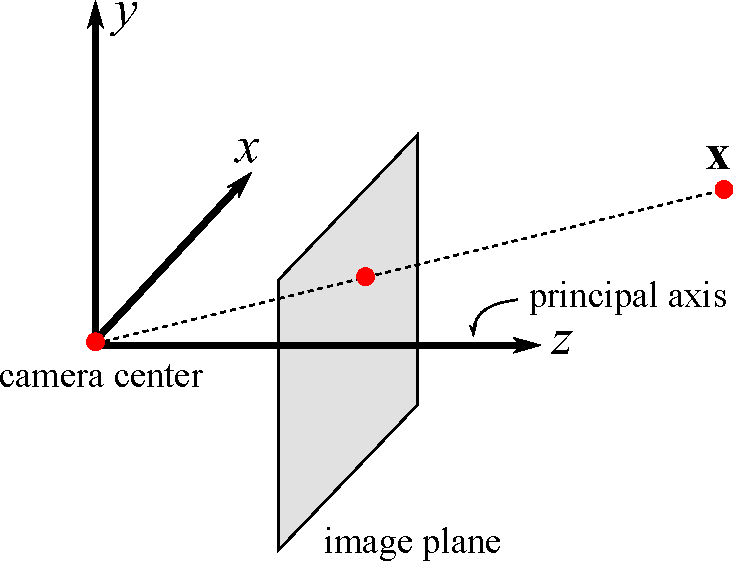
\includegraphics[width=7.5cm]{img/projective_camera.pdf}}
  \caption{Perspective projection of a point $\x$ on the image plane of a camera with camera center in the coordinate system's origin. }
\end{figure}

\subsection{Epipolar geometry}
\label{sec:epi}

% In \cv\ \term{fundamental matrix} represents the relation of points between two stereo images.
Epipolar geometry expresses the geometric constraints encountered when observing a 3D scene by a pair of cameras with known parameters. 
Suppose we choose a point $\x$ on the image of the first camera from such a pair.
The knowledge of its position constraints the position of the corresponding one on the second image.
This point, denoted by $\xd$, lies on the line $\F\x$, where $\F$ is the fundamental matrix.
This line is called \term{the epipolar line}.

\begin{definition}
The \term{fundametal matrix $\F$} for a pair of stereo images is a $3 \times 3$ matrix which satisfies 
\begin{align*}
\xd^T \F \x = 0
\end{align*}
for any pair of corresponding points $\x$ and $\xd$.
\end{definition}

Fundamental matrix for a pair of photos can be estimated from the knowledge of a set of corresponding points since each correspondence is a linear constraint on the values of $\F$. 
Because $\F$ has $9$ real entries and is determined only up to a scaling factor, it has $8$ degrees of freedom and thus at least $8$ correspondences are required to determine its values. 
However, in our case, the matrix is going have only one degree of freedom due to the restrictions we have specified for the input photographs. 
% Since automatic image registration algorithms typically produce more than $8$ correspondences, this

\section{Integral images}

% Later in this work we work with the term of integral images. 
\term{An integral image}, also known as \term{summed area table}, allows fast and efficient computation of a sum of image intesity values inside an arbitrary rectangular area.
A pixel of an integral image represents the sum of all of the original image's pixels that lie to the left and above the considered position: 
\begin{equation*}
\K_I(\x) := \sum_{i \le x} \sum_{j \le y} I(i,j),
\end{equation*}
where $\K$ is the resulting integral image, \emph{I} is the input image image, and $\x = \vect{(x, y)}^{T}$ is a location of a pixel.

An advantage of the integral image is that we are able to compute it using only one pass through the original image. 
Moreover, once we have calculated the integral image, only three integer operations and four memory accesses are required to calculate the sum 
of the original intensities inside any rectangular region (see Figure \ref{fig:integral}).

\begin{figure}[h]
  \label{fig:integral}
  \centering{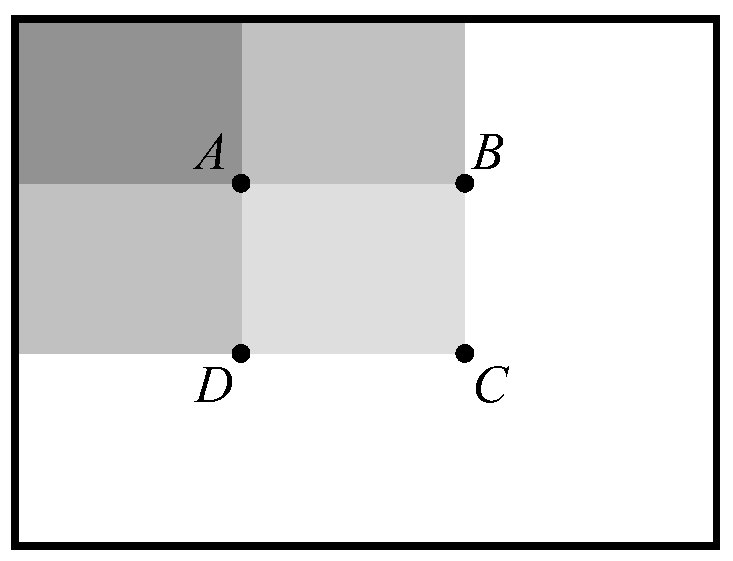
\includegraphics[width=7.5cm]{img/integral_image.pdf}}
  \caption{The sum of any rectangular region can be calculated by only three additions: $C - D - B + A$.}
 \end{figure}




% XXX nedat sem nekam jeste neco o tom, jak vypocitat hloubku z disparity?

% \chapter{Related Work}
In this section we mention some of the approaches that have been proposed earlier. 
We consider algorithms for interest points detection and description especially. 
It gives us an overview of already existing work.

\section{Interest Point Detection}
In 1988, Chris Harris and Mike Stephens \cite{harris1988} published their corner detector based on combining corner and edge detector. 
Although this approach is not scale–invariant, it is widely used nowadays. 

However, many computer vision tasks deal with the real world input data images where objects appear in different ways depending on the scale. 
Due to this fact, Lindberg came out with automatic scale selection for feature detection \cite{lindberg1998}.

There are several other approaches that have been introduced such as edge–based region detector by Jurie and Schmid \cite{jurie2004} or salient region detector by Kadir and Brady \cite{kadir2001}.
But apparently they are not used that much. It seems that due better results and stability, most popular are Hessian–based detectors.

Another example of Hessian–based detector is a detector published by Herbert Bay et al.\  in Speeded–Up Robust Features \cite{surf2006}. 
This detector is partly inspired by SIFT algorithm, but it is several times faster and more robust against the scale transformation and the image rotation. 
It relies on the approximation of determinant of the Hessian matrix that can be computed using integral images. 
Hence, the computation is very fast (see the previous chapter).

\section{Interest Point Description}
Large number of interest point descriptors were introduced. 
The most common one is scale–invariant feature transform \cite{lowe1999}, SIFT for short. 
This algorithm was published in 1999 by a Canadian computer scientist David G. Lowe. 
The descriptor is computed from the intensities around the key point locations where the local gradient direction of picture intensities gives description of the local key point.



\chapter{Image Processing Algorithms}
\label{chap:algorithms}

In this chapter, we introduce the image processing algorithms often applied in software solutions with functionality similar to those discussed in Chapter \ref{chap:overview}. 
Applications reconstructing depth information from photographs or video sequences typically have at their core an algorithm that detects and tracks image primitives (such as corners, blobs, lines, individual pixels, etc.) across several photos/frames. 
This knowledge allows one to estimate the camera parameters, which in turn makes it possible to compute the spacial parameters of the tracked primitives.
% Tohle je asi moc velke rozpatlavani, takze jsem to ani nedopsal: For example, the solution outlined in \todo{reference na Snavelyho} extracts certain image features from individual input photos, matches these features between pairs of photos to obtain tracks, then proceeds to estimate camera parameters and 3D positions of points correponding to these features and finished by visualizing the resulting \pc.

The approaches to computing correspondences between pairs of photos can be divided into \term{sparse correspondence} and \term{dense correspondence} algorithms. 
In the former, a relatively conservative subset of only the most stable \term{features} are considered and paired. 
In the latter, the objective is to obtain a correspondence in the second image for (almost) every pixel of the first image. 
% Thus, dense correspondence algorithms allow us to obtain full diparity map of the first image in the image pair. 
% We can either aim to establish correspondences between a restricted set of primitives, for example just the most stable looking corners detected in the images, or we can aim to establish a correspondence from (almost) every pixel of the reference image. 
% The former approach is called \term{sparse correspondence problem} 

We describe two techniques solving the sparse correspondence problem -- the SIFT \cite{lowe1999} and SURF \cite{surf2006} feature detectors/descriptors -- and then discuss the Lucas-Kanade method for computing optical flow. % XXX ten optical flow je nuten do toho zasadit nejak vic 

% We describe three techniques -- the SIFT feature detector/descriptor, the SURF feature detector/descriptor, and the Graph-cut algorithm. \todo{potrebujeme urcite pridat citace}
% SIFT and SURF are the most used algorithms to detect features.
% Both of them are robust to scale and rotation.
Generally, sparse feature matching algorithms first extract features from each photo. % from a pair of photos of the same scene. % TODO nejsem si jisty, jestli tam napsat "of the same scene", protoze taky mohou byt pouzity k object detection 
If the feature detection is \term{repeatable}, most of the features should be detected in all images where the corresponding scene elements are visible.
Then, for each feature a \term{descriptor} is generated, typically a high-dimensional vector. 
This descriptor is constructed in a way ensuring invariance to various image transformations. 
For instance, the SIFT descriptor is invariant to translation, rotation, scaling, and image noise. 
Thus, applying any of those transformations to the image should leave the descriptors unaffected, making it possible to match image features using Euclidean metric. 
The SIFT descriptor is also partially invariant to illumination changes and to affine transformations, the latter enabling us to perform matching of images capturing the scene from slightly different viewpoints.
% Achieving full invariance to projective transformations is typically too computationally prohibitive.  
% Usually, a descriptor is affinely invariant, meaning .
% Hence for a feature from different viewpoints should be generated the same vector.
% Since the descriptors are computed, we can match them between a pair of images. 
% Due to the fact that our descriptors are vectors, we can match them according to the distance in the space, using Euclidean distance for example.
 
\section{Scale-Invariant Feature Transform}

The scale-invariant feature transform (SIFT) was introduced by Lowe in \cite{lowe1999}, building on a previous work by Lindeberg \cite{lindeberg1998}. 
The paper describes both a feature detector and descriptor. 
To this day, SIFT remains a popular choice for applications such as panorama stitching and object detection. 
It is able to detect objects in images even in the presence of clutter.

Let us outline the major steps in which the algorithm proceeds in its task to repeatably generate a set of features in an image and to compute their corresponding descriptors. 
Recall that an imporant and desirable property of these descriptors is their invariance to image transformations like rotation, scaling or illumination changes. 
% The algorithm starts by building the scale-space of the image. 
Firstly, candidate features are detected over all scales of the grayscale version of the input image. 
Locations of these features are then determined with subpixel precision. 
Simultaneously, features corresponding to unstable image regions are filtered out from the dataset. 
  % Then, for each potential feature, its location and scale model is determined with subpixel precision by fitting a quadratic function.
  % This quadratic functions is also used to filter out unstable features that lie on an edge or are likely to result from image noise. 
In the next stage, each feature is assigned its orientation and scale based on the prevailing gradient directions in the image neighbourhood. 
This orientation is used to establish a reference frame for the construction of the descriptor.
The last step is the feature description.
The SIFT feature descriptor is a 128-dimensional vector determined by the gradients around the feature at the corresponding scale. 
Since the computation of the descriptor is performed using the abovementioned local reference frame, 
the resulting descriptor is invariant to transformations that affect this reference frame in a covariant manner but only partially invariant to affine transformations and illumination changes.
We now proceed to describe both the detection and the descriptor construction steps in more detail.

The first step in the feature detection part of the algorithm is to identify candidate locations of all scales in a highly repeatable manner. 
For this, Gaussian scale-space is employed. 
Recall its definition from Section \ref{sec:gaussder}:
\[
L(x, y; \sigma) = g(x, y, \sigma) * f(x, y),
\]
where $\sigma$ is the deviation of the Gaussian function, $*$ the convolution operator, $f(x, y)$ is the input image, and $g(x, y)$ the Gaussian function
\[
 g(x, y, \sigma) = \left( \frac{1}{\sqrt{2\pi \sigma _1^{2}}} \cdot e^{-\frac{x^{2}+y^{2}}{2\sigma_1^{2}} } \right).
\]

To extract the features in the scale-space we detect the local extrema in the difference-of-Gaussian function $D(x, t, \sigma)$.
The difference-of-Gaussian (DoG) is defined as the difference of two neighbouring images of the scale-space: 
\[
 D(x, y, \sigma) = L(x, y; 2\sigma) - L(x, y; \sigma) = (g(x, y, 2\sigma) - g(x, y, \sigma)) * f(x, y).
\]
Each sample point of the DoG is compared to its eight neighbours in the current scale and nine neighbours on the levels below and above.
If it is larger than all of these neighbours, it is selected as a maximum; if it is smaller than all of them, it is selected as a minimum. 
It can be shown that the DoG approximates the Laplacian of the image at the particular location. 
These extrema should therefore correspond to ``blobs'' in the image.
The application of scale-space ensures that blobs of all possible sizes are detected. 
These locations are taken as an initial set of candidate feature. 

We need to filter this set significantly to ensure high repeatability of the resulting set of features. 
Usually, the detection of scale-space extrema results is a large number of candidate keypoints. 
However, some of them are local extrema resulting from image noise or the responses of the operator along edges. 
Such structures are unstable and should be discarded from the set of candidate keypoints.
To reject such unstable features, we fit a 3D quadratic function to the local sample points and interpolate the location of the extremum.
This is done using quadratic Taylor expansion of the function $D(x, y, \sigma)$ around the detected point.
By calculating the minimum we get the position of the local extremum with a subpixel precission.
Properties of this quadratic function are used to reject unstable extrema: if the function is too shallow, we discard the feature as a result of image noise; if it is too narrow, the extremum likely corresponds to an edge in the image.  
Otherwise we accept it as a feature.

% orientation:
To achieve invariance to rotation, local orientation must be determined for each feature. 
First, we compute a histogram of orientations of image gradients around the its location. 
The peaks of the histogram represent the dominant orientations. 
The orientation corresponding to the highest peak is assigned to the feature. 
If there are several peaks of magnitude within 80\% of the highest peak, multiple keypoints are generated -- one for each such orientation.

The descriptor is then constructed by considering several histograms in the four quadrants of the reference frame of the keypoint.
Typically, each quadrant is divided into four subregions. 
In each of the resulting sixteen subregions, we construct a histogram of orientations of gradients sampled regularly in the subregion. 
Concatenating the values in these histograms results in a 128-dimensional vector.

\section{Speeded-Up Robust Features}

Another popular feature detector/descriptor is the Speeded Up Robust Features (SURF) algorithm, introduced by Bay et al. \cite{surf2006}. 
It is influenced by the SIFT algorithm described above and is based on Hessian-matrix approximation and the computation of Haar wavelet responses. 
The major stages are to detect the features, estimate their orientation and then to each of them assign a descriptor.
Similarly to SIFT, keypoints are again detected in a scale-space to achieve invariance to scaling.
In this approach, however, the scale-space is not constructed explicitly and integral images are employed instead to decrease the computation time. 

The SURF feature detection is based on detecting blob structures using Gaussian kernels.
It uses the Hessian matrix of the convolution of the image with the second derivative of Gaussian.
The determinant of this Hessian expresses the local change around the area.
The points that are simultaneously local extrema of both the determinant and the trace of the Hessian matrix are chosen as candidate keypoints.
%The detection of interest points is performed using an approximation of the Hessian-matrix.

However, the convolution is very costly to calculation time.
It is approximated and speeded-up with the use of integral images and approximated kernels (\ref{sec:integral_images}).
In this way the algorithm is very fast.

The SURF algorithm does not build the scale-space by explicit down-sampling the images.
To detect the features across scales SURF uses larger and larger Gaussian kernels.
The larger Gaussian kernel is used, the more down-sampled image is investigated.

Similarly to SIFT, the SURF descriptor is a vector describing the distribution of intensity values within the neighbourhood of the keypoint. 
The difference lies mainly in the fact that the SURF descriptor is constructed using Haar wavelet responses around the point of interest. % TODO skutecne sum? mozna mi neni jasne, v jakem smyslu
The Haar wavelet responses can be calculated efficiently with integral images again.
Before the descriptor calculation, to be invariant to image rotation it is needed to determine the orientation. 
By determining a unique orientation for a interest point, it is possible to achieve rotational invariance. 
Before the descriptor is calculated the surrounding area of the detected feature is rotated to its direction.

The SURF descriptor describes the surrounding area of the feature.
This area is divided to 4 $\times$ 4 subareas.
To each of these subareas the Haar wavelet responses are calculated in the $x$ and $y$ directions and then are described by the vector
$$v = (\sum{d_x}, \sum{d_y}, \sum{|d_x|}, \sum{|d_y|}),$$
where  $d_x$ and $d_y$ are the wavelet responses in $x$ and $y$ directions.
Concatenating this for all $4 \times 4$ subregions gives $64$-dimensional vector descriptor.

Matching the SURF descriptors between two images can be speeded-up by including the trace of the Hessian (Laplacian) to the process of finding corresponding keypoints. 
We exploit the sign of Laplacian that distinguishes bright blobs on dark background from the reverse situation. 
In the matching stage we compare only features if they have the same sign – type of contrast. 
This costs no additional computation time since this quantity has already been computed at a previous stage.




\section{SIFT vs. SURF}
Both SIFT and SURF are popular feature descriptors based on the distribution of intensity around the interest point.
SURF has been shown to have similar performance to SIFT, but being much faster.
The work \cite{surf2006} highlights the fast computation of the descriptor.
The element enabling this speed-up are the approximations using integral images. 
Also, the SURF descriptor is a 64-dimensional vector, enabling faster computation of the Euclidean distance between the descriptors compared to the 128-dimensional SIFT descriptors.
However, the performance depends on many factors.
The results of comparing and testing SIFT against SURF can be found in \cite{siftsurf2001} and \cite{siftsurf2009}.

In this \cite{siftsurf2001} study the robustness of SIFT and SURF was tested under several different conditions.
It was shown that SIFT and SURF gives similar results when testing the robustness to rotation, illumination and noise 
(the performance of both SIFT and SURF rapidly  decreased on the images with ``salt and pepper" noise).
When testing the viewpoints, two images available in the dataset taken from different viewpoints were chosen and in this case SIFT outperformed SURF.
In general matching the results show that all SIFT and SURF descriptors perform well on all datasets.


In \cite{siftsurf2009} is shown that SIFT still outperform SURF in scale, rotation and blur, but is slow and not good at illumination changes.
SURF gives the best results in computational time and when testing illumination, but it is not stable to rotation and illumination changes. 
This shows that none of these detectors/descriptors is best for all deformation.
Choosing the method mainly depends on the application.

Both of the studies have similar results except the calculation time.
While in \cite{siftsurf2001} was SIFT the most efficient, in \cite{siftsurf2009} the SURF was the fastest.


% \section{Max-flow dense correspondence algorithm}

% In computer vision there is a general task of stereo correspondence.
% It is a problem of discovering the closest match between points of two pictures typically taken from different positions.
% Presumably, rectification of the images considerably simplifies the situation. 
% Sometimes this constraint can be done.
% Once the correspondences are solved, we obtain a disparity map and it can be exploited to reconstruct the positions and distances of the cameras.

% TODO: Nasledujici patri do uvodu kapitoly a taky jsem to tam presunul. 
% Generally, there are two approaches to find the corresponding points.
% One of them is to detect features and interest points in an image and then find corresponding points in the other one.
% Only these high distinctiveness points are matched, hence it is called sparse stereo matching.
% The second way, dense stereo matching, is to match as many pixels as possible.

% In 1999, Roy published an algorithm %\cite{roy1998} 
% \cite{roy1999} to solve the stereo correspondence problem formulated as a maximum-flow problem in a graph.
% It solves efficiently maximum-flow and gives a coherent minimum-cut that presents a disparity surface for the whole image.
% This way provides more accurate depth map then the classic algorithms and the result is computed in shorter time in addition.

%The matching space is defined as a projective 3-d volume (to allow pyramids as well as cubes) formed

\section{Lucas-Kanade algorithm for optical flow} 

Optical flow algorithms are typically applied in postprocessing software for movies to track an object through a video sequence. 
We can think of this problem as the image correspondence problem optimized for the situation where there is very little camera movement between the registered pair of photos, as is in the case with two consecutive frames of a video sequence. 
The output of such algorithm is an array of $2$-dimensional vectors $\mathbf{d}_\x$, where $\x$ is an image position, with the property that the point $\x$ on the first frame corresponds to the point $\x + \mathbf{d}_\x$ on the second one. 
Optical flow is typically not constrained by epipolar geometry, since the assumption is that the video is of a dynamic scene that includes objects moving relative to the camera and each other.
The algorithms for optical flow tend to work only when the differences between the images are significantly limited and the registration can be performed only on a small neighbourhood of the original position of a feature. 

We now describe a classical Lucas-Kanade method \cite{lucas} for calculating the optical flow between two images $I_1$ and $I_2$.

The method proceeds by specifying linear constraints on the values $\mathbf{d}_\x$ and then solves the resulting over-determined system in the least squares sense. 
For each pixel $\x$ that is being tracked, we consider the following equation: 
\begin{align} 
\label{optfloweq} 
\Delta I_1(\x) \cdot \mathbf{d}_\x = I_1(\x) - I_2(\x),
\end{align} 
where $\Delta I_1(\x)$ is the image gradient at $\x$.
% $$\Delta I_1(\x) = \Big(\imd1{\partial x}(\x), \imd1{\partial y}(\x)\Big).$$
This is motivated by the observation that the apparent movement should be roughly in the direction of the image gradient for locations with a large jump of the intensity value between the frames. 
On the other hand, when the intensity of a pixel is approximately the same in both frames, we either expect no movement or just a movement perpendicular to the image gradient.
However, the inclusion of just the above equations does not enforce spatial consistency of the movement in any way.
This is taken into account by repeating equation (\ref{optfloweq}) for each position $\x^i$ taken from the neighbourhood of $\x$ of a fixed size. 
Specifically, we add the following equation for each $\x^i$:
$$\Delta I(\x^i) \cdot \mathbf{d}_\x = I_1(\x^i) - I_2(\x^i).$$
Note that the differences are read from the position $\x^i$ while the movement constrained is of the pixel $\x$.
Solving the above over-determined system using conventional methods gives us the desired values $\mathbf{d}_\x$.
% Optical flow is calculated for every pixel of the video frame, meaning that the output is a field of $2$-dimensional vector $d_\x$ (for each pixel $\x$ of the image) determining the movement of the pixel between the two frames of the video. 


\chapter{Developing for Android}
\label{chap:android}

Android, Inc\@. was founded in October in 2003 by Andy Rubin, Rich Miner, Nick Sears, and Chris White. 
At first, the company planned to develop an operating system for digital cameras % but when they realised that the market is not large enough,
but ultimately % they decided to change their intentions and 
decided to focus on smartphones instead. % operating system.
% That time, the Apple's iPhone was not released yet. 
% The rival mobile phones operating systems were Symbian and Windows Mobile.
% After four years with the financial aid of Google, Android was revealed.
HTC Dream, the first phone with the Android operating system, was sold in autumn 2008.
Majority of Android's code is released under a free license. 
This allows developers to modify and (with certain exceptions) freely distribute the software.
Due to this, Android became the most popular operating system for smartphones.
In this chapter, we introduce this system from programmer's perspective and give a brief description of how to implement an Android application.
The purpose of the chapter is to highlight the main architectural differences between Android and conventional desktop platforms rather then providing a complete programer's manual. 

\section{Introduction to the Android development}

% Android is a product of \term{The Open Handset Alliance}, which develops open standards for mobile devices and is led by Google.
The Android platform is a layered environment built on the foundation of the Linux kernel.
It includes a user interface library featuring various types of elements (views, windows, display boxes, lists, etc.),  
an embedded web browser, and support for OpenGL ES.
Most Android-powered devices have built-in sensors to measure, e.g., motion, orientation or temperature. 
These include an accelerometer, a gyroscope or a barometer.
It also provides an array of connectivity options, for example Wi-Fi, Bluetooth or cellular data.
A built-in camera support is also included and most Android handsets indeed feature a camera. 
% In an effort to improve graphics, the Android platform supports an environment for 2D and 3D graphics development including OpenGL library.
The data storage support is provided by SQLite, a relational database management system in the form of a library implementing self-contained and server-less SQL database engine.
 
Linux kernel, the first architectural layer of the platform, is used for memory and process management, device drivers, and networking.
Above this, we have the native libraries, which include graphics support, media codecs, SQLite, and WebKit.
These are written in C or C++ and called through a Java interface.
The actual applications are running on the Dalvik Virtual Machine (DVM), an implementation of the Java Virtual Machine optimized for low processing power and memory resources.
% We should note that the virtual machine applications are running within is not Java virtual machine, but Dalvik Virtual machine.
The Android Runtime Layer consists of this DVM and the core Java libraries. 

The next level is the Application Framework, which manages functions fundamental to running applications.
Its major part is formed by the Activity Manager (managing the life cycle of the applications) and various Content Providers (managing data sharing between the applications).
Other notable parts are the Telephony Manager (handling voice calls), the Location Manager (specifying location using GPS or cell tower) and the Resource Manager.
The final layer is formed by the individual applications.
Some of them are preinstalled and provided by Google while the rest are third party applications created by the community.
The structure of the system is illustrated in Figure \ref{fig:architecture} below.
\begin{figure}[h!]
    \centering{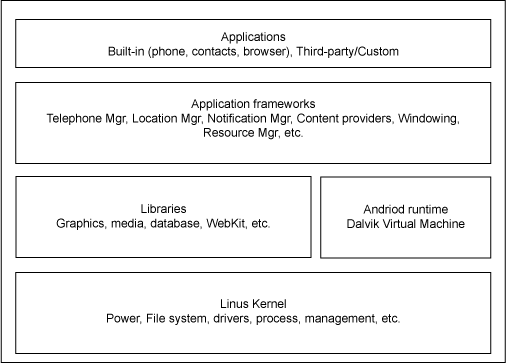
\includegraphics[width=80mm]{img/software_layers.png}}
    \caption{The architecture of the system.} 
    \label{fig:architecture}
\end{figure}

Android applications are written in the Java programming language and run within an instance of the Dalvik Virtual Machine.
A key part of the application is the AndroidManifest\@.xml file containing installation meta-data, including the necessary permissions.
An example of such permission is the ability to use the phone's camera or to access the Internet.
\begin{figure}[h!]
    \centering{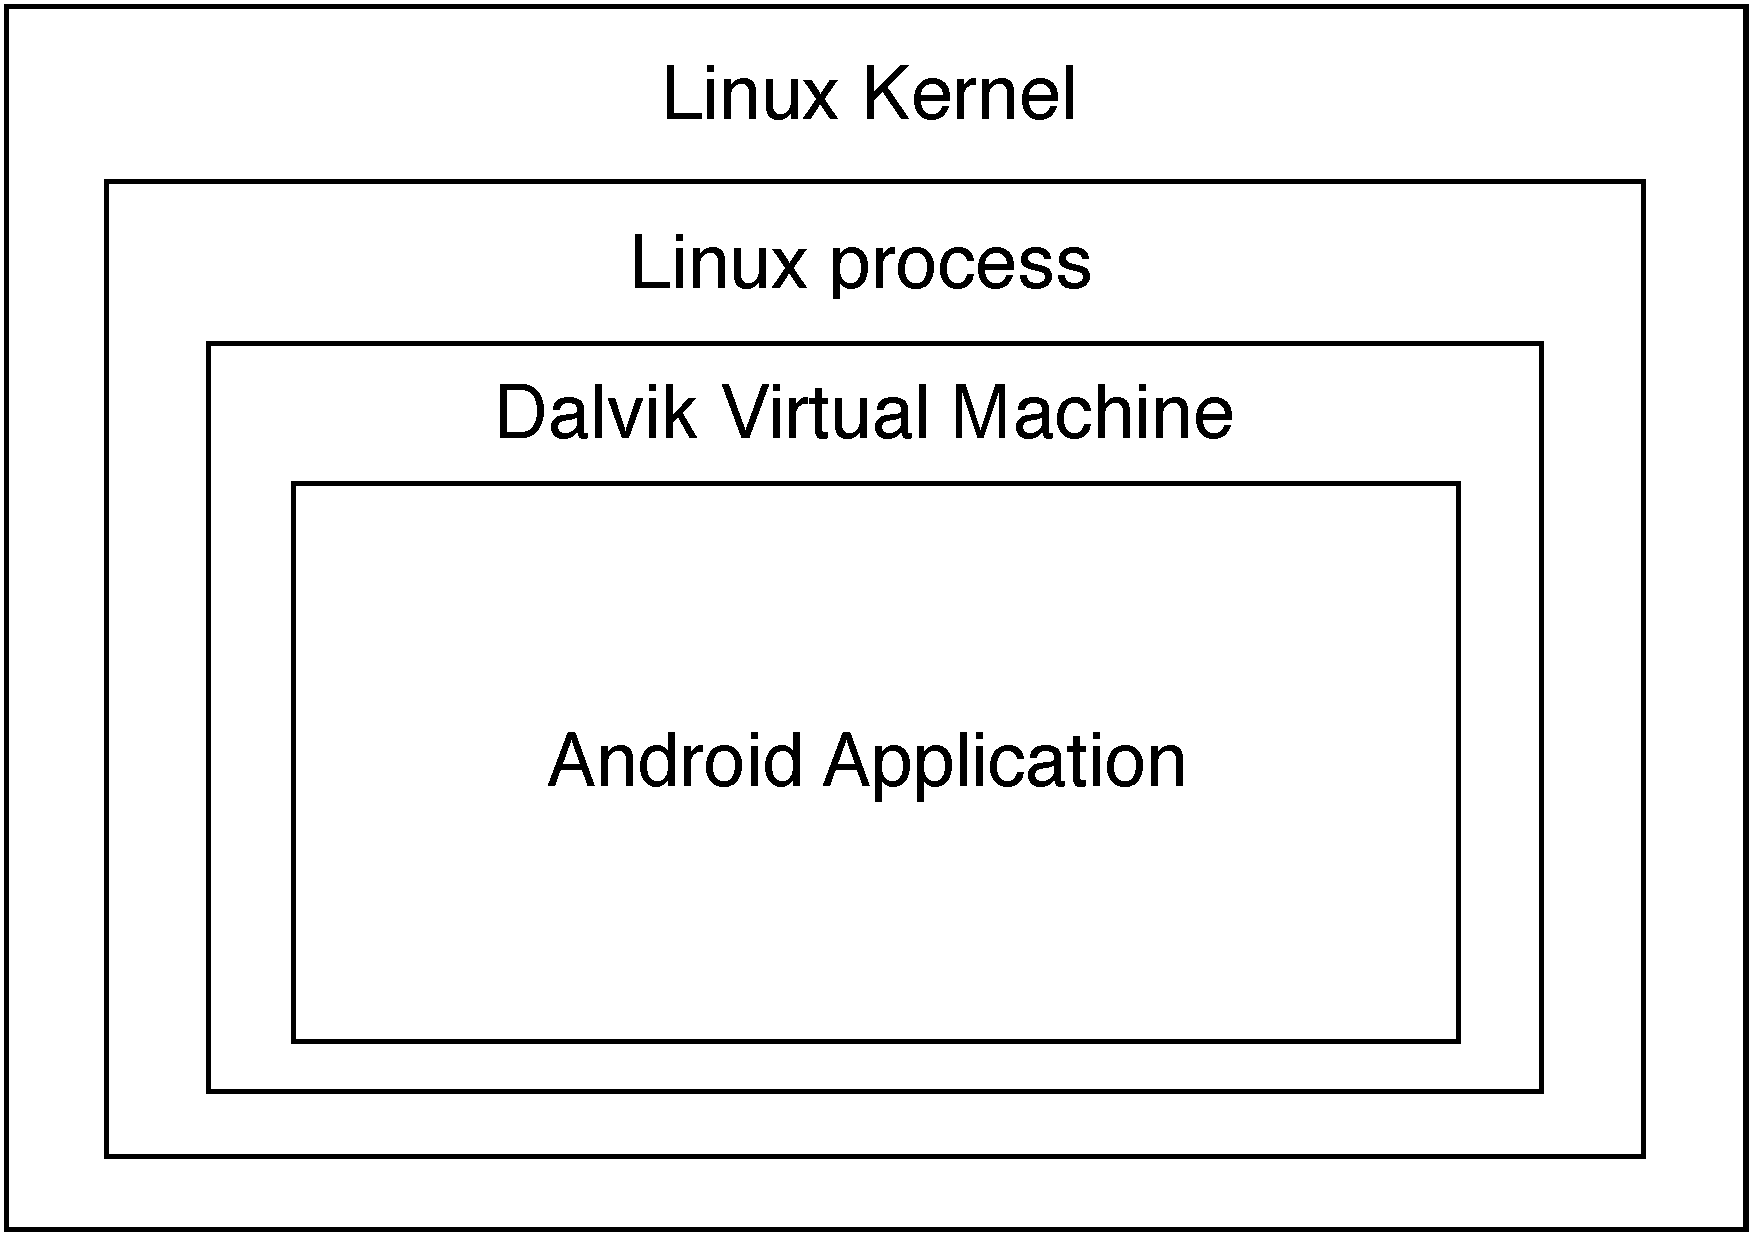
\includegraphics[width=80mm]{img/dalvik.pdf}}
    \caption{A typical Android application runs within an instance of the Dalvik Virtual Machine.}
\end{figure}

The tools required for the development of an Android application are the Android Software Development Kit (SDK)\footnote{\url{http://developer.android.com/sdk/}} and a Java IDE, such as Eclipse\footnote{\url{http://www.eclipse.org}} or the Android Studio\footnote{\url{http://developer.android.com/sdk/installing/studio.html}} based on IntelliJ IDEA. 
The Android SDK contains an Eclipse plugin supporting Android developement, documentation, sample code, and various tools, such as the Android Debug Bridge used by the programmer to communicate with an application running on a device or an emulator. 
% % \item The Android SDK is provided as \@.zip file including Java archive file containing all necessary classes to build an application (android\@.jar),
% the SDK documentation, a directory with sample code, Android Debug Bridge and other tools needed to build an application.

% TODO: tohle pripadne pridejme az ten text bude vyladenejsi: In the rest of this chapter we describe some of the implementational parts of the application development. 

\section{Application components}

Compared to the situation on the majority of conventional platforms, Android interacts with the running applications in a much closer manner. 
Actually, the system expects a certain specific architectural structure of the application expressed using concepts from object oriented programming. 
A typical Android application is be decomposed into several classes, each being a descendant of a particular class provided by the SDK. 
Through this, requirements on what and how the application's class has to implement are imposed. 
This approach allows, e.g., sophisticated interaction between different applications running on the same phone. 
For example, one application can use a list of contacts maintained by another application without the developers of the latter having to set up any protocols or data exports -- they only need to obey the software development principles of the platform. 
Thanks to this, the user data are seamlessly protected from an unauthorised access by the system through the principle of least privilege. 
In the above-mentioned example, the access to the list of contacts would not be granted unless it is listed in the accessing application's manifest file and this requirement has been authorized by the user. 
Since these properties of the platform are rather unique, we devote this section to discuss them. 

An Android application is built from several components typically belonging to one of the following groups: 
\begin{itemize}
\item{activities,}
\item{services,}
\item{content providers, etc.}
\end{itemize}

\term{An activity} can be thought of as a UI screen providing elements such as views, lists, buttons, labels, etc. along with the implementation of their functionality.
The layout of an activity and the widgets placed in the window is described in a separate XML file. 
Most applications consist of more than one activity with one being designated as the main one.
Although the activities form one application, they are all independent from each other.
If another application has a permission to do so, it can start an activity of a different app.
From the developer's perspective, activities are represented by classes descending from the Activity class defined in the SDK. 

\term{A service} is a component used to perform operations in the background.
For example, if the application needs to run a long-term computation, the user can switch to another application with the computation continues. 

\term{A content provider} manages sharing data across applications.
When the app is storing data, for example in the file system or an SQLite database, the content provider interface can be used to access or even modify the data from other applications. 

The platform utilizes additional classes of components besides the above-mentioned ones (e.g., broadcast receivers). 
However, we omit them for the sake of brevity. 

%%% docteno sem 
The interaction between various components and activities is facilitated by \term{intents.} 
An intent is a message to the system to invoke new activity, service or broadcast.
% It is a component activating mechanism in Android.
The reader is referred to the Android SDK documentation for more information about activities, services, content provides, intents, etc. 

\section{Activity lifecycle}
\label{sec:lifecycle}

During its life cycle, an application switches between different application states.
Compared to desktop platforms, the programmer has only limited control over these state transitions.
On the desktop computer, the developer has a certain level of control over, e.g., minimizing or closing a window of an application or quitting the software. 
This cannot be affected on the discussed platform. 
The life cycle is a collection of functions the operating system executes on the application during its runtime. 

There are five stages of the life of an application:
\begin{itemize}
\item the starting state,
\item the running state,
\item the paused state,
\item the stopped state,
\item and the destroyed state.
\end{itemize}

The starting state and the destroyed state are phases of the activity when it is not in the memory.
To launch the app, the main activity class's \emph{onCreate()} method is called and eventually the application transitions into the running state.
When in a running state, the application is actually on the screen visible to the user and handling all user interactions such as typing or touching the screen. 
An activity in this state has the highest priority for memory allocation in the activity stack.
It is killed by the operating system only in extreme situations.
This transition from starting to running state is the most expensive operation in terms of battery requirements.
That is also the reason why Android does not destroy every activity when it gets to the background, 
because it is probable that it is going to be used again. 

\begin{figure}[h!]
    \centering{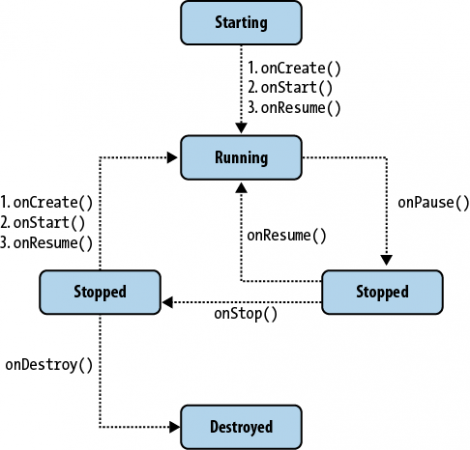
\includegraphics[width=80mm]{img/life_cycles.png}}
    \caption{Life cycle of an application.}
\end{figure}

The application is paused (in a paused state) when not interacting with user but is still visible on the screen.
This state does not occur very often, since most applications cover entire screen.
However, in the cases when the application is partly visible yet not interacting with the user, the pause state is utilized. 

When the application is not visible but still in memory, it is in a stopped state.
Then, it is easy to bring it up to the front again or it can be destroyed and thus removed from the memory.

\section{User interface}
\label{sec:ui}

All elements of the application's user interface are built using a hierarchy of \term{View} and \term{ViewGroup} objects.
The layout describing the visual structure of the \term{Views} is declared in a separate XML file.
Although not recommended, the user interface can be also declared explicitly in the source code. 
There are two principal layouting options: \term{LinearLayout} arranges the inner elements in a single row or a column,
while \term{RelativeLayout} positions the elements in relation to their parent or each other.

With the layout defined, the developer can then utilize the UI elements offered by the SDK, such as menus, action bars, dialogs or toasts.
There are several types of menus such as options menu or context menu. 
The options menu displays a collection of buttons when the user taps the menu button typically available on an Android device. 
From the Android version 3\@.0 higher, the options menu items are included in the action bar after touching the action overflow button. 
The context menu is a floating menu associated with a particular element in a view displayed after touching the element.

Action bars provide a way for navigating through the application's interface. 
The action bar is located at the top of an activity and can display the activity title, icon or other actions and items.
Some Android devices have a hardware action overflow button which opens the options menu at the bottom of an activity. 
Action bars are superior to the options menus since an action bar is always visible while options menu shows only on the user request.

A dialog is a small window informing the user about some action. 
Unlike \term{toast} it usually requires the users action before continuing by confirmation or giving some additional information.
The \term{toast} provides only feedback about some action in a small pop-up that disappears after a moment.

\section{Sensors}

Most Android devices have built-in motion, environmental and positional sensors.
Motion sensors are sensors measuring the rotation along three axes and give us an opportunity to detect motion, shaking or tilting of the device. 
Environmental sensors are applied for measuring temperature, illumination, or humidity.
Built-in magnetometers and orientation sensors provide information about the current position and/or orientation of a device and can be used in applications for GPS navigation or in mapping software. 
The sensor events are access using an instance of the \term{SensorManager} class.

\section{Data storage}

There are several possibilities for storing application data in Android. 
The internal storage is preferable when we do not want other applications to access them. 
The read and write operations are performed using instances of \term{FileInputStream} and \term{FileOutputStream}.

However, media files such as pictures, video files or audio records are expected to be shared and accessible from other applications.
In such a case, the external storage is utilized through methods of the \term{Environment} class.
The function \term{getExternalStoragePublicDirectory()} depending on the supplied argument returns the path of the root directory where we can write our data, for example: 
\begin{itemize}
\item{../Music/,}
\item{../Pictures/,}
\item{../Movies/,}
\item{../Download/,}
\item{etc.}
\end{itemize}
As an argument we pass the type of the directory we want to access, for example \term{Environment\@.DIRECTORY\_MUSIC}.

\section{Example} 

In this section, we illustrate the concepts from the above sections on an example application. 
As noted in the beginning of the chapter, this is not intended to be an all-encompassing description of creating an Android application. 
Rather, it is supposed to illustrate crucial parts the process. 

A user interface, discussed in Section \ref{sec:ui}, is typically specified using an XML file stored in the \term{/res/layout} directory.
Below is a simple example of such file: 

\begin{lstlisting}
    <?xml version="1.0" encoding="utf-8"?>
    <RelativeLayout xmlns:android="http://schemas.android.com/apk/res/android"
        xmlns:tools="http://schemas.android.com/tools"
        android:layout_width="match_parent"
        android:layout_height="match_parent">
    
        <org.opencv.android.NativeCameraView
            android:id="@+id/camera_view"
            android:layout_width="match_parent"
            android:layout_height="match_parent"/>
        
        <RelativeLayout
    	    android:layout_width="200dp"
    	    android:layout_height="match_parent"
    	    android:layout_margin="10dp"
    	    android:layout_centerInParent="true">
    	    
            <Button
    	        android:id="@+id/captureButton"
    	        android:layout_width="90dp"
    	        android:layout_height="90dp"
    	        android:layout_alignParentBottom="true"
    	        android:layout_centerHorizontal="true"
    	        android:background="@drawable/circle_button"
    	        android:onClick="callTakePicture"/>
            
            <Button
    	        android:id="@+id/startCapturingButton"
    	        android:layout_width="90dp"
    	        android:layout_height="90dp"
    	        android:layout_alignParentBottom="true"
    	        android:layout_centerHorizontal="true"
    	        android:background="@drawable/circle_button"
    	        android:onClick="start_stopAutoCapturing"
    	        android:visibility="invisible"/>
    	          
    	    <ToggleButton
    	        android:id="@+id/toggleAutoCaptureButton"
                    android:layout_width="wrap_content" 
                    android:layout_height="wrap_content" 
                    android:layout_alignParentTop="true"
                    android:layout_centerHorizontal="true"
    	        android:textOn="AutoCapture on"
    	        android:textOff="AutoCapture off"	    
    	        android:onClick="autoCaptureStateChanged"/>
    
    	    <TextView
    	        android:id="@+id/startCapturing_textView"
    	        android:layout_width="wrap_content"
    	        android:layout_height="wrap_content"
    	        android:layout_above="@+id/captureButton"
    	        android:layout_centerHorizontal="true"
    	        android:text="@string/startcapturing_text"
    	        android:visibility="invisible"/>
    
    	</RelativeLayout>
    	
    </RelativeLayout>
\end{lstlisting}

In our example, the root element is a \term{RelativeLayout} element which allows us to describe a relative position with respect to the parent. 
Inside the \term{RelativeLayout}, we find \term{org.opencv.android.NativeCameraView} which is an element of the OpenCV library used for camera view and another \term{RelativeLayout} with \term{Buttons}, a \term{ToggleButton} and a \term{TextView}.
All of the elements have their width and height specified by using the \term{android:layoutwidth} and \term{android:layoutwidth} attributes.
The value of these attributes can be \term{matchparent} or \term{wrapcontent} or a specific number of units.

It is possible to define a specific layout of an activity for a particular screen orientation through supplying an alternative XML file of the same name in the \term{res/layout-land} folder.

In the \term{src} folder, we have all the .java files representing activities or classes.
Every Android application has at least one ``main'' activity invoked by the system when the application is launched.
Due to the activity lifecycle (see Section \ref{sec:lifecycle}), it is necessary to implement the following methods:
\begin{itemize}
\item \term{onCreate()},
\item \term{onPause()},
\item \term{onResume()}.
\end{itemize}

Usually only the basic startup actions are completed in the \term{onCreate()} method, for example setting up the layout or initializing some of the class variables.
The implementation of the \term{onCreate()} method in the example below first invokes the ancestor's corresponding method, then initializes the layout using the \term{setContentView()} method and then performs some application specific processing. 
\begin{lstlisting}
    @Override
    public void onCreate(Bundle savedInstanceState) {
        super.onCreate(savedInstanceState);
        setContentView(R.layout.activity_gallery);
        
        adapter = new Adapter(this);
        ArrayList<GridImage> db_update = new ArrayList<GridImage>();
        for (String s : files) {
          ...
        }
        ...
    }
\end{lstlisting}
Depending on the needs of our application, we can add some code into the other overriding methods handling the activity lifecycle: 
\begin{lstlisting}
    @Override
    public void onPause(){
        super.onPause();
        ...
    }
  	
    @Override
    public void onResume(){
        super.onResume();
        ...
    }
\end{lstlisting}
To make the user interface interactive we need to assign functions to be executed when tapping on the individual elements.
This can be done either in the XML file by specifying the activity's method name in an attribute of the corresponding element: 
\begin{lstlisting}
    <Button  
      ...
      android:onClick="takePicture"
      ... />
\end{lstlisting}
Alternatively, the action can be assigned in the code:
\begin{lstlisting}
    Button my_button = (Button)findViewById(R.id.button);
    my_button.setOnClickListener( new View.OnClickListener() {
      ...    
    });
\end{lstlisting}



















\chapter{OpenCV}

OpenCV (a short for Open Source Computer Vision) is an open source library covering the area of \cv.
It was designed mainly for real-time applications and computational efficiency.
OpenCV is written in C and C++, can take advantage of multicore processors and \todo{abychom si touhle zminkou ale nenabehli a nekdo se neptal, jak pouzivame na tom androidu parallelismus}
runs on various platforms including Linux, Windows, and Mac OS X.
Bindings for Python, Matlab and other programming languages have been introduced as well. 
% TODO tohle jsou spis obecne vety patrici nekam do uvodu, kde je taky nejspis uz mame: 
% 	Nowadays, computer vision is widely used in many parts of computer science.
% 	We should notice that it is increasingly being used for images and video for the web applications.
% 	For example camera calibration and image stitching techniques are applied to street-map images such as in Google's Street View.
% TODO tohle je zbytecne zminovat znovu o par vet dal: As we already mentioned, OpenCV is mainly aimed at real-time applications and computational efficiency. 
% TODO v tuhle chvili asi neni zasadni: If we are interested in further optimization we can achieve it by installing Integrated Performance Primitives (IPP), that consist of low-level optimized routines and are used automatically by OpenCV when the library is installed.
% OpenCV provides an environment to create vision applications more easily and more effective and sophisticated.
OpenCV contains over 500 functions spanning many areas of \cv, for example medical imaging, camera calibration, robotics or stereo vision.

\section{The Origin of OpenCV}

OpenCV was developed by Intel and the first alpha-version was released in 1999.
At first, the project was an Intel Research initiative to advance CPU-intensive applications, part of a series of projects including real-time ray tracing and 3D display walls.
That time, several university groups developed open computer vision infrastructure, code that every student could reach and use to his or her own vision application.
This code was adapting by the students, building on the top what was implemented before.
When one of the OpenCV authors noticed this, OpenCV was conceived as a way how to create computer vision infrastructure universally available.

The team developing OpenCV included experts from Russia (e.g. Vadim Pisarevsky) and Intel's Performance Library Team.  
The goals supporting the reason why to concern with this research were to provide not only open but also optimized code for computer vision,
disseminate knowledge about computer vision by providing easily accessible open library and to advance vision-based commercial applications.

The first 1.0 version was released in 2006.
From 2008 OpenCV is supported by Willow Garage, who are notable for their Robot Operating System.
As of today, the latest version of OpenCV is 2.4.5 released in the April of 2013.

\todo{tady ted zase rikame neco, co bych cekal bud maximalne v uvodnim odstavci}
Since the first release, OpenCV has been used in many applications. 
It has even been used in sound and music recognition area where the vision techniques were applied to sound spectrogram images.

\section{Structure of OpenCV}
OpenCV consist of image processing functions and algorithms and because computer vision and machine learning often go hand-in-hand, 
OpenCV also contains Machine Learning Library(MLL).
This part of OpenCV library is focused on statistical pattern recognition and clustering. 

Basically, we can structure OpenCV into four components, illustrated on Figure \ref{fig:opencvstruc}.
First of all, it would be the CXCore component containing the basic data structures and operations on them.
The HighGUI component ensures I/O routines and functions for loading and storing images.
ML is the machine learning library. 
Finally, the Computer Vision component containing basic image processing and vision algorithm.
\begin{figure}[h!]
    \label{fig:opencvstruc} 
    \centering{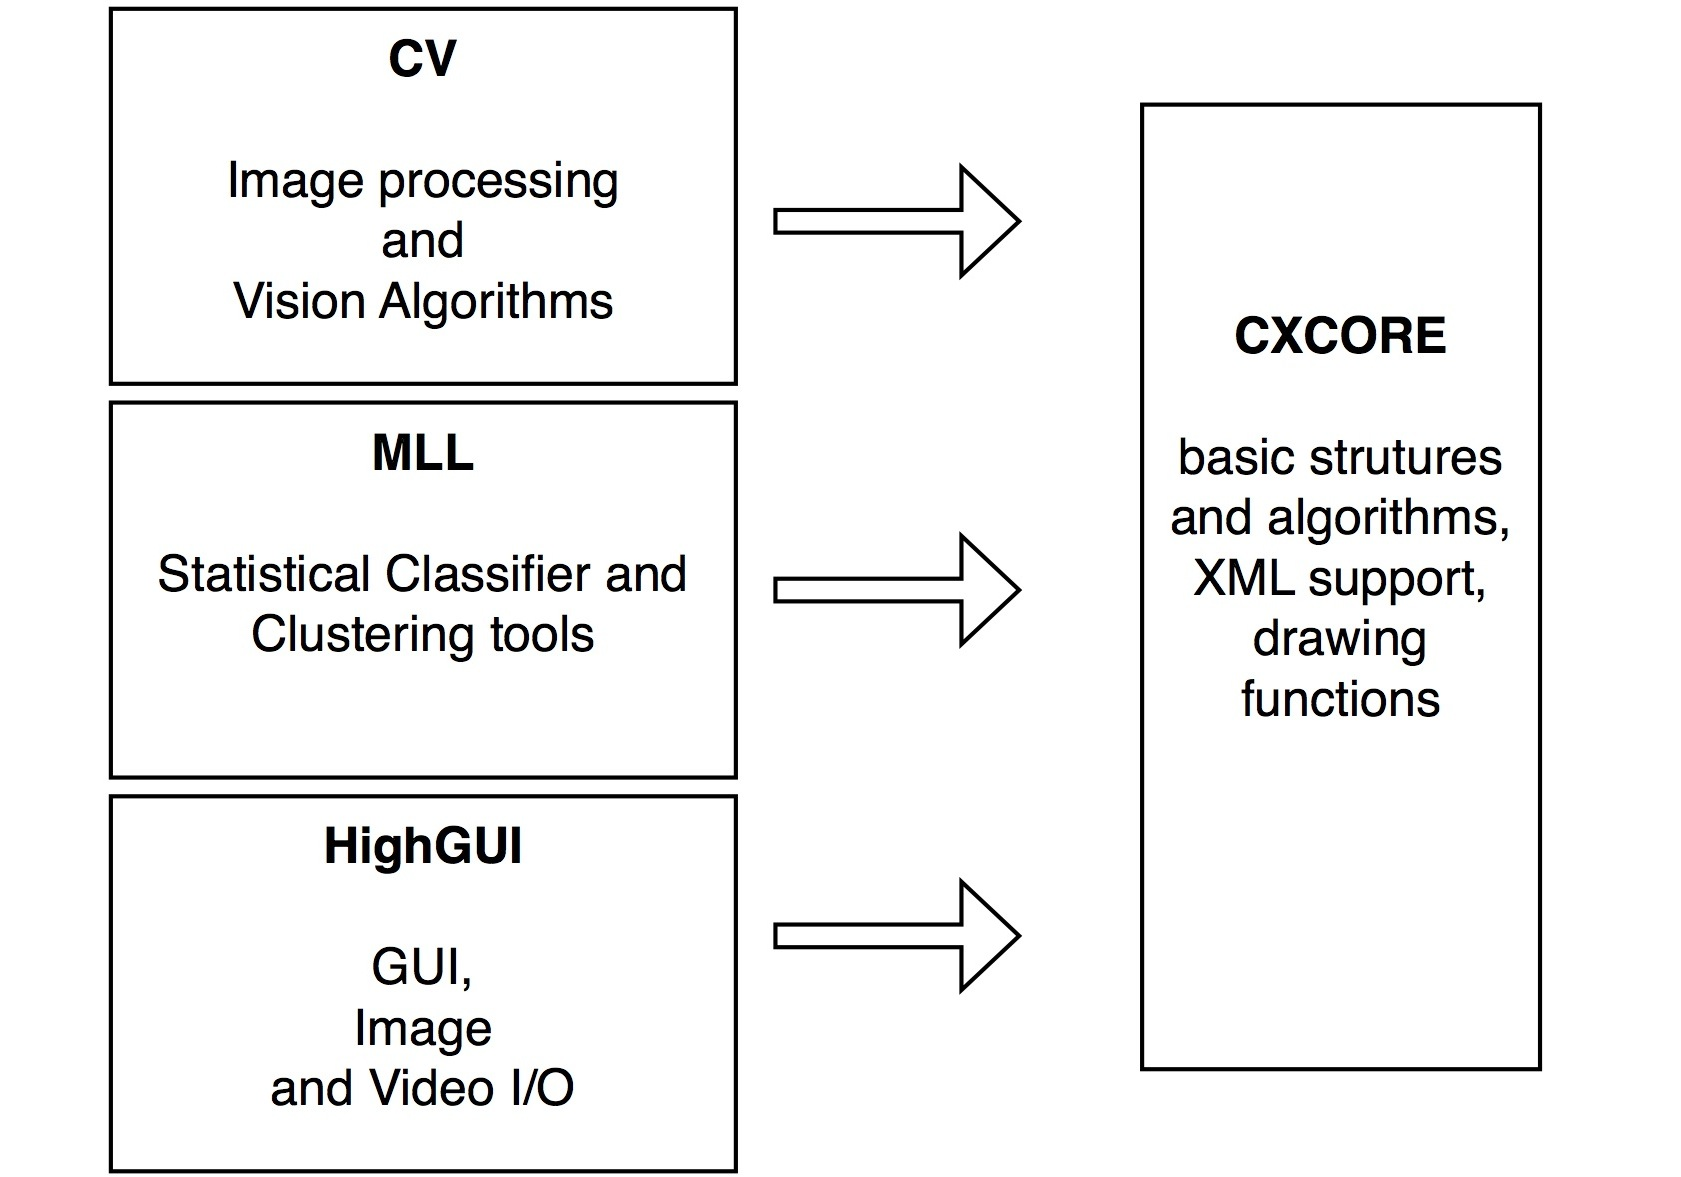
\includegraphics[width=110mm]{img/opencv_structure.jpg}}
    \caption{The basic structure of OpenCV library.}
\end{figure}
CXCore provides the core functionality including \todo{ten seznam prosim predelejme tak, aby byl spravne typograficky: mala pismenka a carky na konci radku krome posledniho zakonceneho teckou}:
\begin{itemize}
  \item Basic Structures
  \item Operations on Arrays
  \item Dynamic Structures
  \item Drawing Functions
  \item XML/YAML Persistence
  \item Clustering and Search in Multi-Dimensional Spaces
  \item Utility and System Functions and Macros.
\end{itemize}

In this part of OpenCV library we can find the basic structures that are needed for image processing.
They are represented as structures in the class Basic Structures. For example \stype{CvPoint} defines a point, \stype{CvSize} is a set of two numbers representing size of rectangle, 
\stype{CvScalar} is a container of double values, \stype{IplImage} is a structure inherited from the Intel Image Processing Library designed for loading images, 
or \stype{CvMat} is a data structure for storing a matrix.

As we can presume, the basic methods to work with these structures are implemented.
We can find there functions for mathematical operations on matrices such as multiplication (\stype{void cvMul()}), transposition (\stype{void cvTranspose()}), or
others like dividing multi-channel array into several single-channel arrays (\stype{void cvSplit()}).

Available are also drawing functions working with matrices or images including \stype{void cvCircle()} which as arguments takes an image, centre point of the circle,
and a colour and draws a circle in the image. Similarly \stype{void cvEllipse()} or \stype{void cvDrawContours()}.


The section with functions for image processing and computer vision provides these functionalities:
\begin{itemize}

  \item Image Filtering
  \item Geometric Image Transformations
  \item Miscellaneous Image Transformations
  \item Histograms
  \item Feature Detection
  \item Motion Analysis and Object Tracking
  \item Structural Analysis and Shape Descriptors
  \item Planar Subdivisions
  \item Object Detection
  \item Camera Calibration and 3D Reconstruction

\end{itemize}


\section{OpenCV4Android}
OpenCV library was written in C and this makes it portable to almost any commercial system.
Since the version 2.0, OpenCV includes also the new interface written in C++. \todo{predchozi vetu nevim proc rikame v sekci o androidu}
Later also wrappers for languages such as Java or Python have been developed. 
Since 2010 OpenCV was also ported to the Android environment, it allows to use the full power of the library in the development of mobile applications.
\todo{vubec cely tenhle odstavecek se hodi spis na zacatek kapitolky} 

In comparison with desktop version it also includes the \stype{opencv.android} package containing all the additional functions for the Android platform.
This package provides mainly an environment for work with camera by offering classes such as  \stype{NativeCameraView.java} or  \stype{CameraBridgeViewBase.java}.


\chapter{Implementation}
\label{chap:implementation}

This chapter is devoted to the implementation of our software.
The result of this work is an Android application that allows to take photos with a camera, browse them and pick a pair of images for the resulting 3D model of the disparity map which was calculated from the selected input data.
The expected input data are described in Section \ref{prob}.

Our task was to design an algorithm solving the problem of calculation the depth information from a pair of images on the Android platform.
When implementing the software for Android we are limited to the input data of lower quality.
The Android camera lenses are made of plastic and cause a significant non-linear distortion which can not be easily simulated.
Also, due to the limited capacity of calculation memory of mobile phones we need to down-sample the resolution of the input images.
These problems disallow using common approaches of solving the dens corresponding problem.

In Section \ref{sec:impl_outline} of this chapter we enumerate the subtasks and describe how was our approach designed.
 
\section{Implementation outline}
\label{sec:impl_outline}
In the this section we describe the way how was the task solved, what algorithms were chosen and how was the application implemented.
%To implement the Android application, several subtask must be completed.
%At first it is the graphical user interface and handling the camera which is managed through Android Activities and xml files as we described in chapter \ref{chap:android}.
%Secondly, we deal with the calculation, which consist of the image registration, the keypoint detection, the keypoint matching and solving the dense correspondence problem.

To solve our task, we followed these steps:
\begin{itemize}
\item at first we find the initial relative position of the pair of input images,
\item then we detect and match SURF keypoints from which is chosen the most robust match to specify more accurate relative position,
\item then we detect larger amount of SURF keypoints. The matching process uses the information of the relative position estimated in the previous step,
\item at last, we get the dense correspondences by detecting even more matches using the optical flow algorithm.
\end{itemize}

Finding the initial relative position of the pair of the images is implemented by using Sum of absolute differences (described in Section \ref{sec:metrics}).
At first, we create a scale-space, find the overlap of the images in the lowest scale and by upscaling specify the overlapping area more accurately.
In this way the registration runs in approximately two seconds for a pair of the expected input.

%Image registration (finding the relative position of the pair of the images) is implemented by using Sum of absolute differences (described in \ref{sec:metrics}).
%At first, we create a scale-space from the input pair of images, so we can find relatively fast the overlap with minimal difference of intensities of the image pair by comparing each possible overlap in the lowest scale. 
%When we have the approximate overlap, we take the image of the scale above and try to find better result by shifting the matched area in the 5-pixels range.
%This we repeat until we look over all of the levels of the scale-space or for computational efficiency we estimate the result satisfiable when the width or hight of the investigating scale image is higher then a constant value.
%Because we expect the image input in the size of approximately 1000 $\times$ 800 pixels, for the experiments in our work we set the constant to 200. 

\begin{figure}[h]
\centerline{
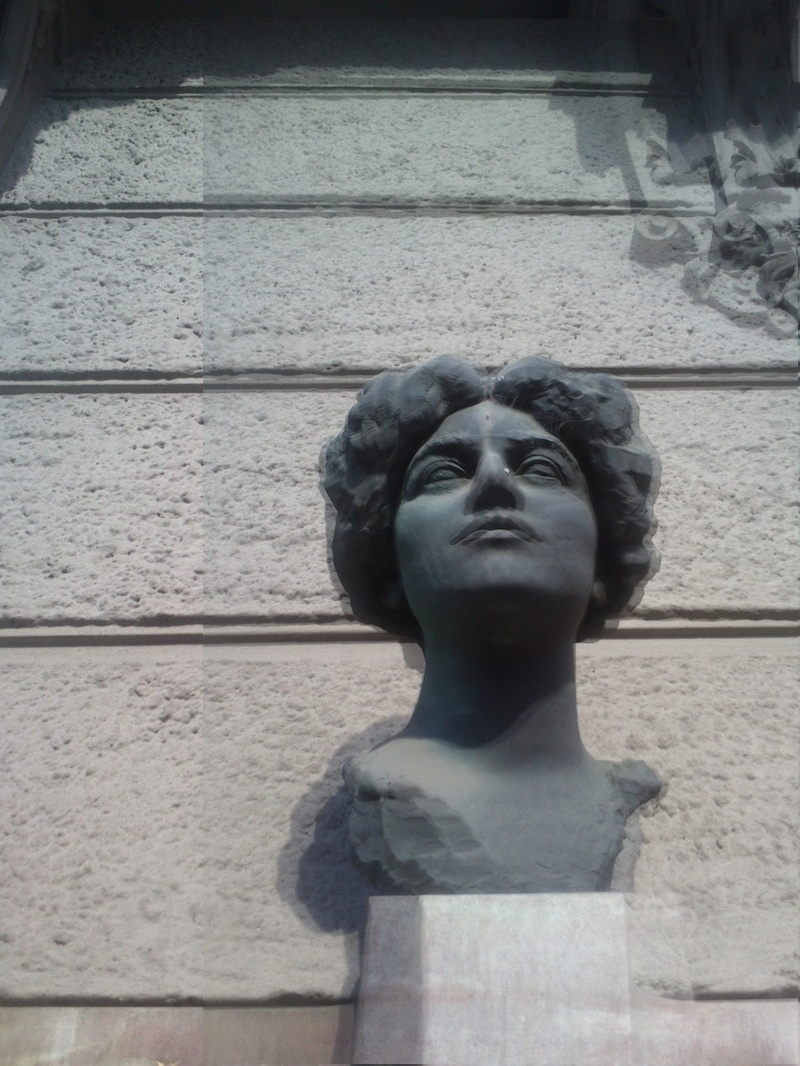
\includegraphics[width=4.5cm]{img/ema_overlap.png}
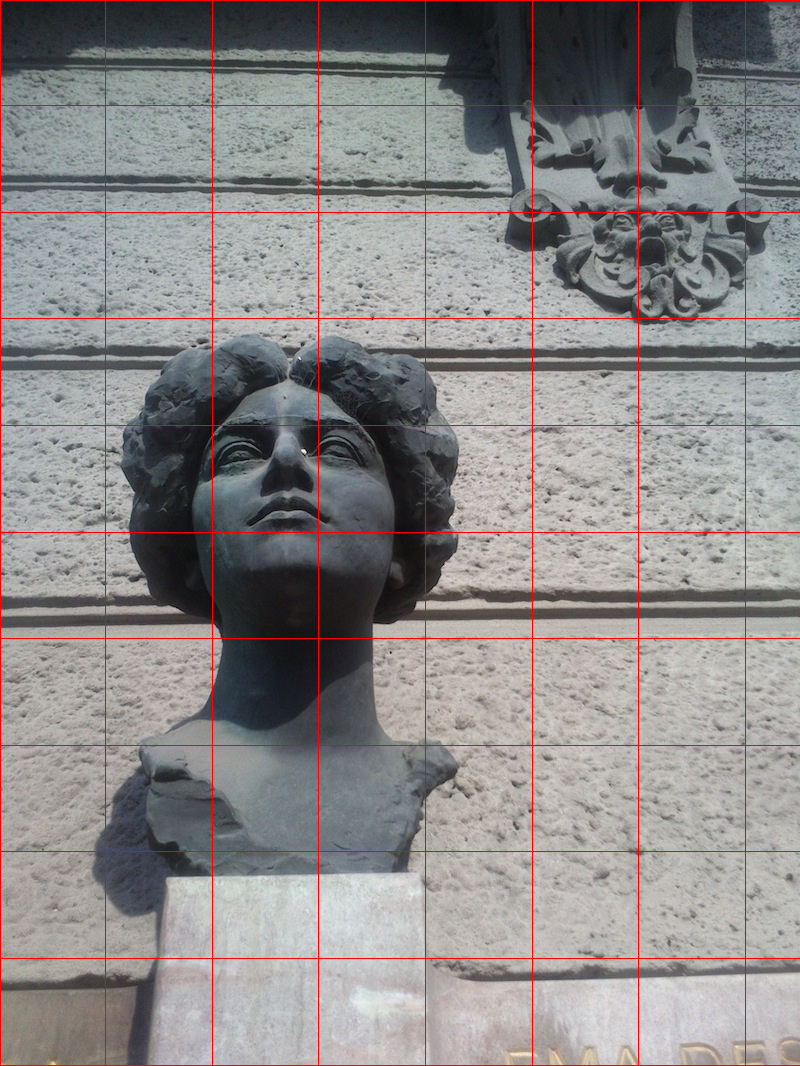
\includegraphics[width=4.5cm]{img/ema_buckets.png}}
\caption{Left: The result of the registration where the process of upscaling was stopped when the height of the image was over 200px. Right: The division of an image into square-boxes.}
\label{fig:overlap_and_buckets}
\end{figure}

The next step of the process is detection of keypoints which are detected with the SURF detector.
We divide the images into square-boxes of the same size and to each square-box we assign an array of keypoints situated in it.
This saves the computational time when finding the match -- instead of comparing every possible correspondence between the images we compare only those which are situated in the square-boxes located in the corresponding areas.
At first we find the most robust match from only the SURF keypoints where the response is higher than 4000.
Based on this match we estimate the direction of the shift which gives us more accurate relative position of the input pair of images.

%The next step of the process is detection of keypoints which are detected with the SURF detector.
%We divide the images into square-boxes of the same size and to each square-box we assign an array of keypoints situated in it.
%Because of the previous calculation of approximate overlap we do not have to match all keypoints in the image, but we choose only the keypoints lying in the overlap.
%To identify the relative position of the image pair better we detect the most robust keypoint match from our SURF keypoint set and calculate the vector defining the direction of the shift of the keypoint.
%To find this robust match we choose only the keypoints with response higher than 4000 and each of them we try to match with one keypoint extracted in the second image but only in the corresponding 30 $\times$ 30 pixels area determined due the previous image registration.
%To decrease the computational time we use the pre-calculated square-boxes to find the keypoints of the second image lying in this area.
%To avoid mismatches we reject the matches where the matched keypoints differs too much in the orientation or if there is more than one obvious potential points for the match.

\begin{figure}[h]
\centerline{
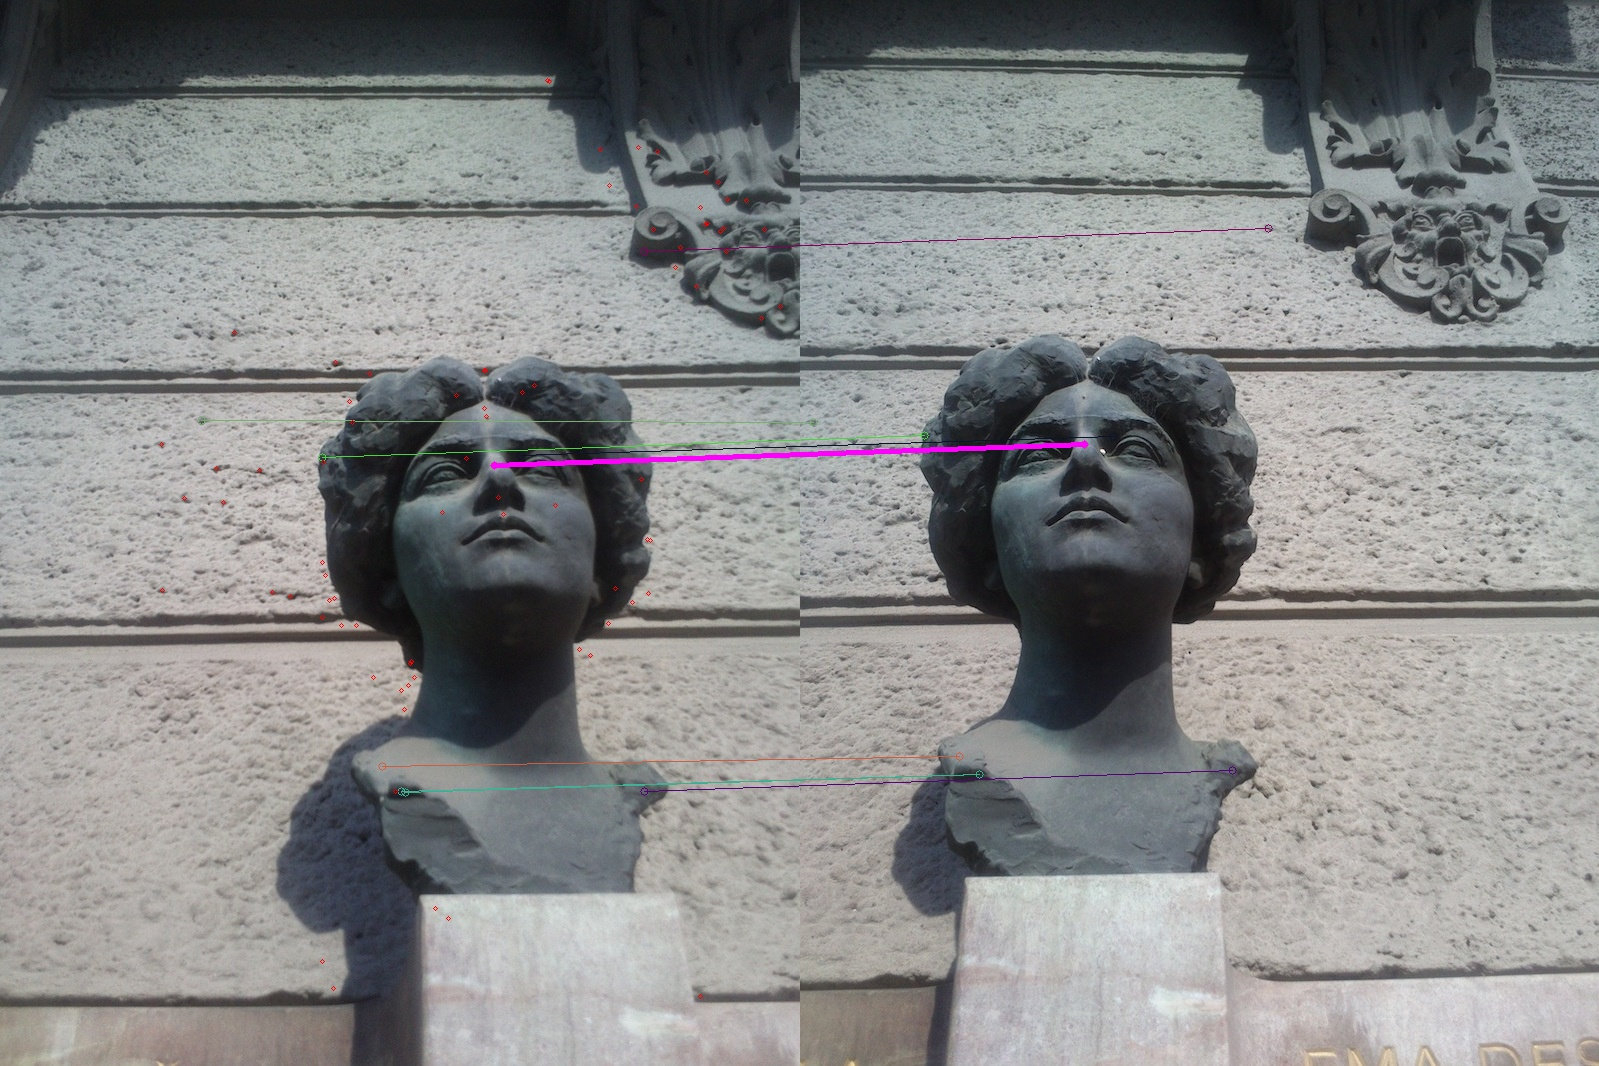
\includegraphics[width=9cm]{img/ema_direction.png}}
\caption{The most robust match chosen from the keypoints with response higher than 4000. According to this match the more accurate relative position of images is estimated.}
\label{fig:robust_match}
\end{figure}

In the next step we match the detected SURF keypoints one more time.
For each keypoint we calculate the corresponding area of the surroundings in the shape of a rectangle oriented in the direction of the shift. 
To avoid mismatches we reject the matches where the matched keypoints differs too much in the orientation or if there is more than one obvious potential points for the match.

%When we know the more accurate relative position of the images, we investigate the keypoints one more time.
%Now we iterate all of them. 
%Each keypoint in the first image we try to match with a keypoint in the estimated corresponding surrounding area in the second image in the shape of oriented rectangle computed based on the more accurate relative image position.
%This oriented rectangle actually consists of two rectangles -- one large and one smaller localised in the middle of the previous one.
%The corresponding keypoint is accepted only if its located in the inner one.
%The size of the larger rectangle is set to 60 $\times$ 120 pixels.
%The inner rectangle after some experiments was set to the 10\% of width and 20\% of height.
%It was shown that it gives better results than only a bit larger window of the the width of 20\% of width and 35\% of height size.
%Matched keypoints which differs too much in the orientation or are not obviously the best match we reject again.
%We can see the comparison in Figure \ref{fig:matching_comparison}.


%Dense correspondence: optical flow::
At this point we have relatively robust matches for sparse correspondence. 
For the calculation of the depth information we need to extract more corresponding points.
Assuming the difference of images is limited, we use for this purpose optical flow algorithm. 
For each SURF keypoint in the first image we detect corners or other features acceptable for the tracking algorithm in its 70 $\times$ 70 pixels area.


Calculating the optical flow we get the corresponding points in the second image.
With high probability some of the results will be influenced by noise.
To avoid these mismatches we calculate the variation of the distances between each match.
If the variation is higher than 300 we discard all of the detected optical flow matches.

The result is visualized in OpenGL ES.
Every keypoint is represented as a triangle in a space with the depth calculated from the correspondence.
At first, the user can view the rough model created from the results of SURF matching.
Each time some of the dense corresponding points are calculated with optical flow algorithm, the model is updated.




% Ukázka použití některých konstrukcí LateXu (odkomentujte, chcete-li)
% %%% Ukázka použití některých konstrukcí LaTeXu

\subsection{Ukázka \LaTeX{}u}
\label{ssec:ukazka}

This short subsection serves as an~example of basic \LaTeX{} constructs,
which can be useful for writing a~thesis.

Let us start with lists:

\begin{itemize}
\item The logo of Matfyz is displayed in figure~\ref{fig:mff}.
\item This is subsection~\ref{ssec:ukazka}.
\item Citing literature~\cite{lamport94}.
\end{itemize}

Different kinds of dashes:
red-black (short),
pages 16--22 (middle),
$45-44$ (minus),
and this is --- as you could have expected --- a~sentence-level dash,
which is the longest.
(Note that we have follwed \verb|a| by a~tilde instead of a~space
to avoid line breaks at that place.)

\newtheorem{theorem}{Theorem}
\newtheorem*{define}{Definition}	% Definice nečíslujeme, proto "*"

\begin{define}
A~{\sl Tree} is a connected graph with no cycles.
\end{define}

\begin{theorem}
This theorem is false.
\end{theorem}

\begin{proof}
False theorems do not have proofs.
\end{proof}

\begin{figure}
	\centering
	
\includegraphics[width=30mm]{../img/logo.eps}
	\caption{Logo of MFF UK}
	\label{fig:mff}
\end{figure}


\chapter*{Conclusion}
\addcontentsline{toc}{chapter}{Conclusion}

We have been testing our application on a Sony ST27i mobile device.
On the testing input data in Figure \ref{fig:input_samples} we obtained satisfiable results as is shown in Chapter \ref{chap:eval}.
For the testing input data, in the case of a bust of Ema Destinová we obtained a 3D model shaping the head and a part of a wall in the background.
In the second case, the input images gave us a result as an inclined plane in the angle of the memorial in the picture.
These results are comparable with the real appearance of the scenes and can be indicated as acceptable results.

Our implementation fails and does not give good results on noisy images or images of chaotic scenes.
In such a kind of scenes the features are matched incorrectly or is not even detected a sufficient number of SURF keypoints to reconstruct the 3D information. 
With high probability, the relative position of a pair of images of different illumination will not be estimated correctly.
Because of the relevant restriction on the area of the shape of an oriented rectangle where are the corresponding points searched (as we explained in Chapter \ref{chap:implementation}),
it is not possible to match the keypoints correctly when the registration fails.

\section*{Future work}

While we use a sum of absolute differences to detect the initial relative position, our approach fails on pairs of images with varying illumination.
Also it does not give good results on the images influenced by noise, which is quite common on the images taken by mobile phone camera, 
especially when the lightening conditions are not ideal.
This can be solved by obtaining the information of relative position by using mutual information while the mutual information is independent to the information of illuminance.

Current version of our program detects the  depth information from a pair of images.
Our implementation could be also extended to the input of $n$ photos. 
It would be necessary to find the relative position of all pairs of images.
This does not have to be calculated explicitly, but possibly we could estimate the position of two images when having the information about their position with the third image.
Detection and matching of SURF keypoints would be applied only to the pairs with an overlapping part.
Most of the implemented methods were designed to be easily extended for this purpose.

For a simple usage of the application we tried to implement an auto-capturing option for taking pictures.
However, we have not managed to optimalize it's behaviour, because it was not the main goal of this work. 
Therefore, it could be an option how to extend the application.
If we go even further, this way of using the device's equipment such an accelerometer can be used to estimate the relative position of taken pictures detected from the motion of the device.
We should note that we can not rely on any interaction with the user to calibrate the camera, since the the mobile phone lens causes a non-linear distortion of the image and non-linear distortion can not be modeled.






%%% Seznam použité literatury
%%% Seznam použité literatury je zpracován podle platných standardů. Povinnou citační
%%% normou pro bakalářskou práci je ISO 690. Jména časopisů lze uvádět zkráceně, ale jen
%%% v kodifikované podobě. Všechny použité zdroje a prameny musí být řádně citovány.

\def\bibname{Bibliography}
\begin{thebibliography}{99}
\addcontentsline{toc}{chapter}{\bibname}

\bibitem{cnnsynth}
  \emph{The 44\textsuperscript{th} President Inauguration.}
  CNN, Inc., 2013. Accessible from \url{http://www.cnn.com/themoment}, 2013.

\bibitem{surf2006}
  {\sc  H. Bay, A. Ess, T. Tuytelaars, and L. Van Gool.}
  \emph{Speeded–Up Robust Features (SURF).}
  In European Conference on Computer Vision, 2006.

\bibitem{ransac}
  {\sc M. A. Fischler and R. C. Bolles.} 
  \emph{Random sample consensus: A paradigm for model fitting with applications to image analysis and automated cartography.} 
  In Communications of the ACM, 1981.

\bibitem{harris1988}
  {\sc C. Harris and M. Stephens.} 
  \emph{A combined corner and edge detector.}
  In Proceedings of the Alvey Vision Conference, 1988.

\bibitem{multipleview}
  {\sc  R. Hartley and A. Zisserman.}
  \emph{Multiple View Geometry in Computer Vision.}
  Cambridge University Press, 2003.

\bibitem{hirschmuller2008}
  {\sc  H. Hirschmüller}
  \emph{Stereo Processing by Semiglobal Matching and Mutual Information.}
  In Pattern Analysis and Machine Intelligence, IEEE Transactions on, 2008.

\bibitem{marketshare}
  IDC Worldwide Mobile Phone Tracker, 2013.

\bibitem{siftsurf2009}
  {\sc L. Juan and O. Gwun.} 
  \emph{A Comparison of SIFT, PCA-SIFT and SURF.}
  In International Journal of Image Processing, 2009.

\bibitem{jurie2004}
  {\sc F. Jurie and C. Schmid.} 
  \emph{Scale–invariant shape features for recognition of object categories.}
  In Conference on Computer Vision and Pattern Recognition, 2004.

\bibitem{kadir2001}
  {\sc T. Kadir and M. Brady.} 
  \emph{Scale, saliency and image description.}
  In International Journal of Computer Vision, 2001.

\bibitem{siftsurf2001}
  {\sc N. Y. Khan, B. McCane, and G. Wyvill.} 
  \emph{SIFT and SURF Performance Evaluation Against Various Image Deformations on Benchmark Dataset.}
  In International Conference on Digital Image Computing: Techniques and Applications, 2001.

  
\bibitem{lindeberg1998}
  {\sc T. Lindeberg.} 
  \emph{Feature detection with automatic scale selection.}
  In International Journal of Computer Vision, 1998.

\bibitem{lowe1999}
  {\sc D. Lowe.} 
  \emph{Object recognition from scale–invariant features.}
  In CCV, 1999.

\bibitem{lucas}
  {\sc B. D. Lucas and T. Kanade. } 
  \emph{An iterative image registration technique with an application to stereo vision.}
  In Proceedings of Imaging Understanding Workshop, 1981.

\bibitem{roy1999}
  {\sc S. Roy.} 
  \emph{Stereo Without Epipolar Lines: A Maximum-Flow Formulation.}
  In International Journal of Computer Vision, 1999.

\bibitem{snavely2008}
  {\sc N. Snavely, R. Garg, S. M. Seitz, and R. Szeliski.} 
  \emph{Finding Paths through the World's Photos.}
  In Journal ACM Transactions on Graphics, 2008.

\bibitem{snavely2007}
  {\sc N. Snavely, S. M. Seitz, and R. Szeliski.} 
  \emph{Modeling the world from Internet photo collections.}
  In International Journal of Computer Vision, 2007.

\bibitem{snavely2006}
  {\sc N. Snavely, S. M. Seitz, and R. Szeliski.} 
  \emph{Photo tourism: Exploring photo collections in 3D.}
  In ACM Transactions on Graphics (SIGGRAPH Proceedings), 2006.

\bibitem{snavely2008}
  {\sc N. Snavely, S. M. Seitz, and R. Szeliski.} 
  \emph{Skeletal graphs for efficient structure from motion.}
  Computer Vision and Pattern Recognition, IEEE Conference on, 2008.

\bibitem{szeliski2010} 
  {\sc R. Szeliski.}
  \emph{Computer Vision: Algorithms and Applications.}
  Springer, 2010. 


\end{thebibliography}


%%% Tabulky v bakalářské práci, existují-li.
% \chapwithtoc{List of Tables}

%%% Použité zkratky v bakalářské práci, existují-li, včetně jejich vysvětlení.
% \chapwithtoc{List of Abbreviations}

%%% Přílohy k bakalářské práci, existují-li (různé dodatky jako výpisy programů,
%%% diagramy apod.). Každá příloha musí být alespoň jednou odkazována z vlastního
%%% textu práce. Přílohy se číslují.
% \chapwithtoc{Attachments}

\openright
\end{document}
